\documentclass{article}
\usepackage{graphicx}
\usepackage{titletoc}
\usepackage{titlesec}
\usepackage{geometry} 
\usepackage{fontspec, xunicode, xltxtra}
\usepackage{float}
\usepackage{cite}
\usepackage{amsmath}
\usepackage{listings}
\usepackage{titletoc}
\usepackage{bm}

\geometry{left=3cm,right=3cm,top=3cm,bottom=3cm}
\DeclareMathOperator*{\argmin}{argmin}
\DeclareMathOperator*{\argmax}{argmax}
\DeclareMathOperator*{\var}{var}
\DeclareMathOperator*{\expec}{E}

\begin{document}
\title{\textsf{Homework 4 for Pattern Recognition}}
\author{Fan JIN\quad (2015011506)}
\maketitle

\section*{Question 1}
{
    \subsection*{Visualization}
    {
        \begin{figure}[H]
            \centering
            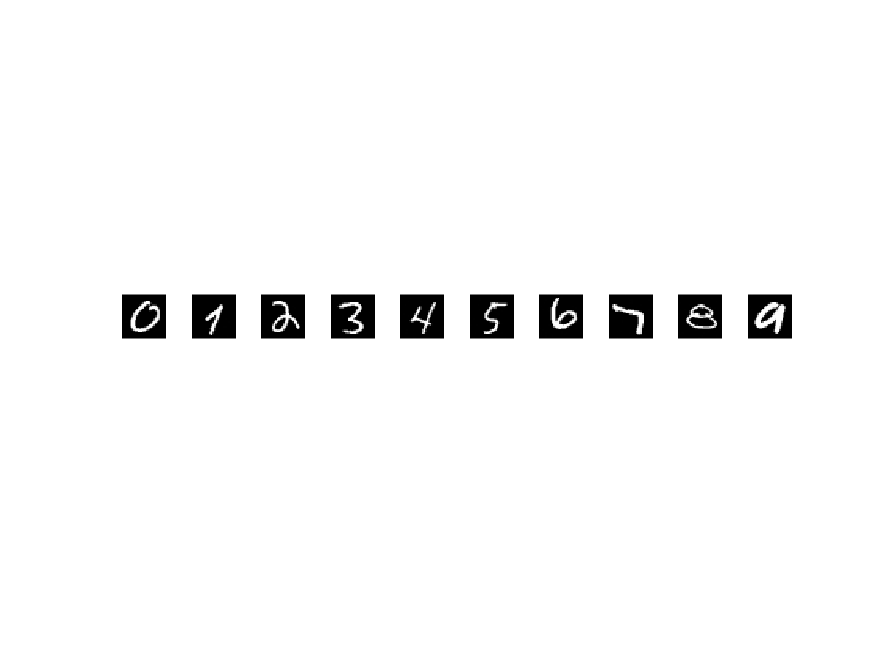
\includegraphics[width = 1.0\linewidth]{src1/glance.png}
            \caption{A glance at all the 10 categories}
        \end{figure}
    }

    \subsection*{Confusion Matrices}
    {
        \begin{figure}[H]
            \centering
            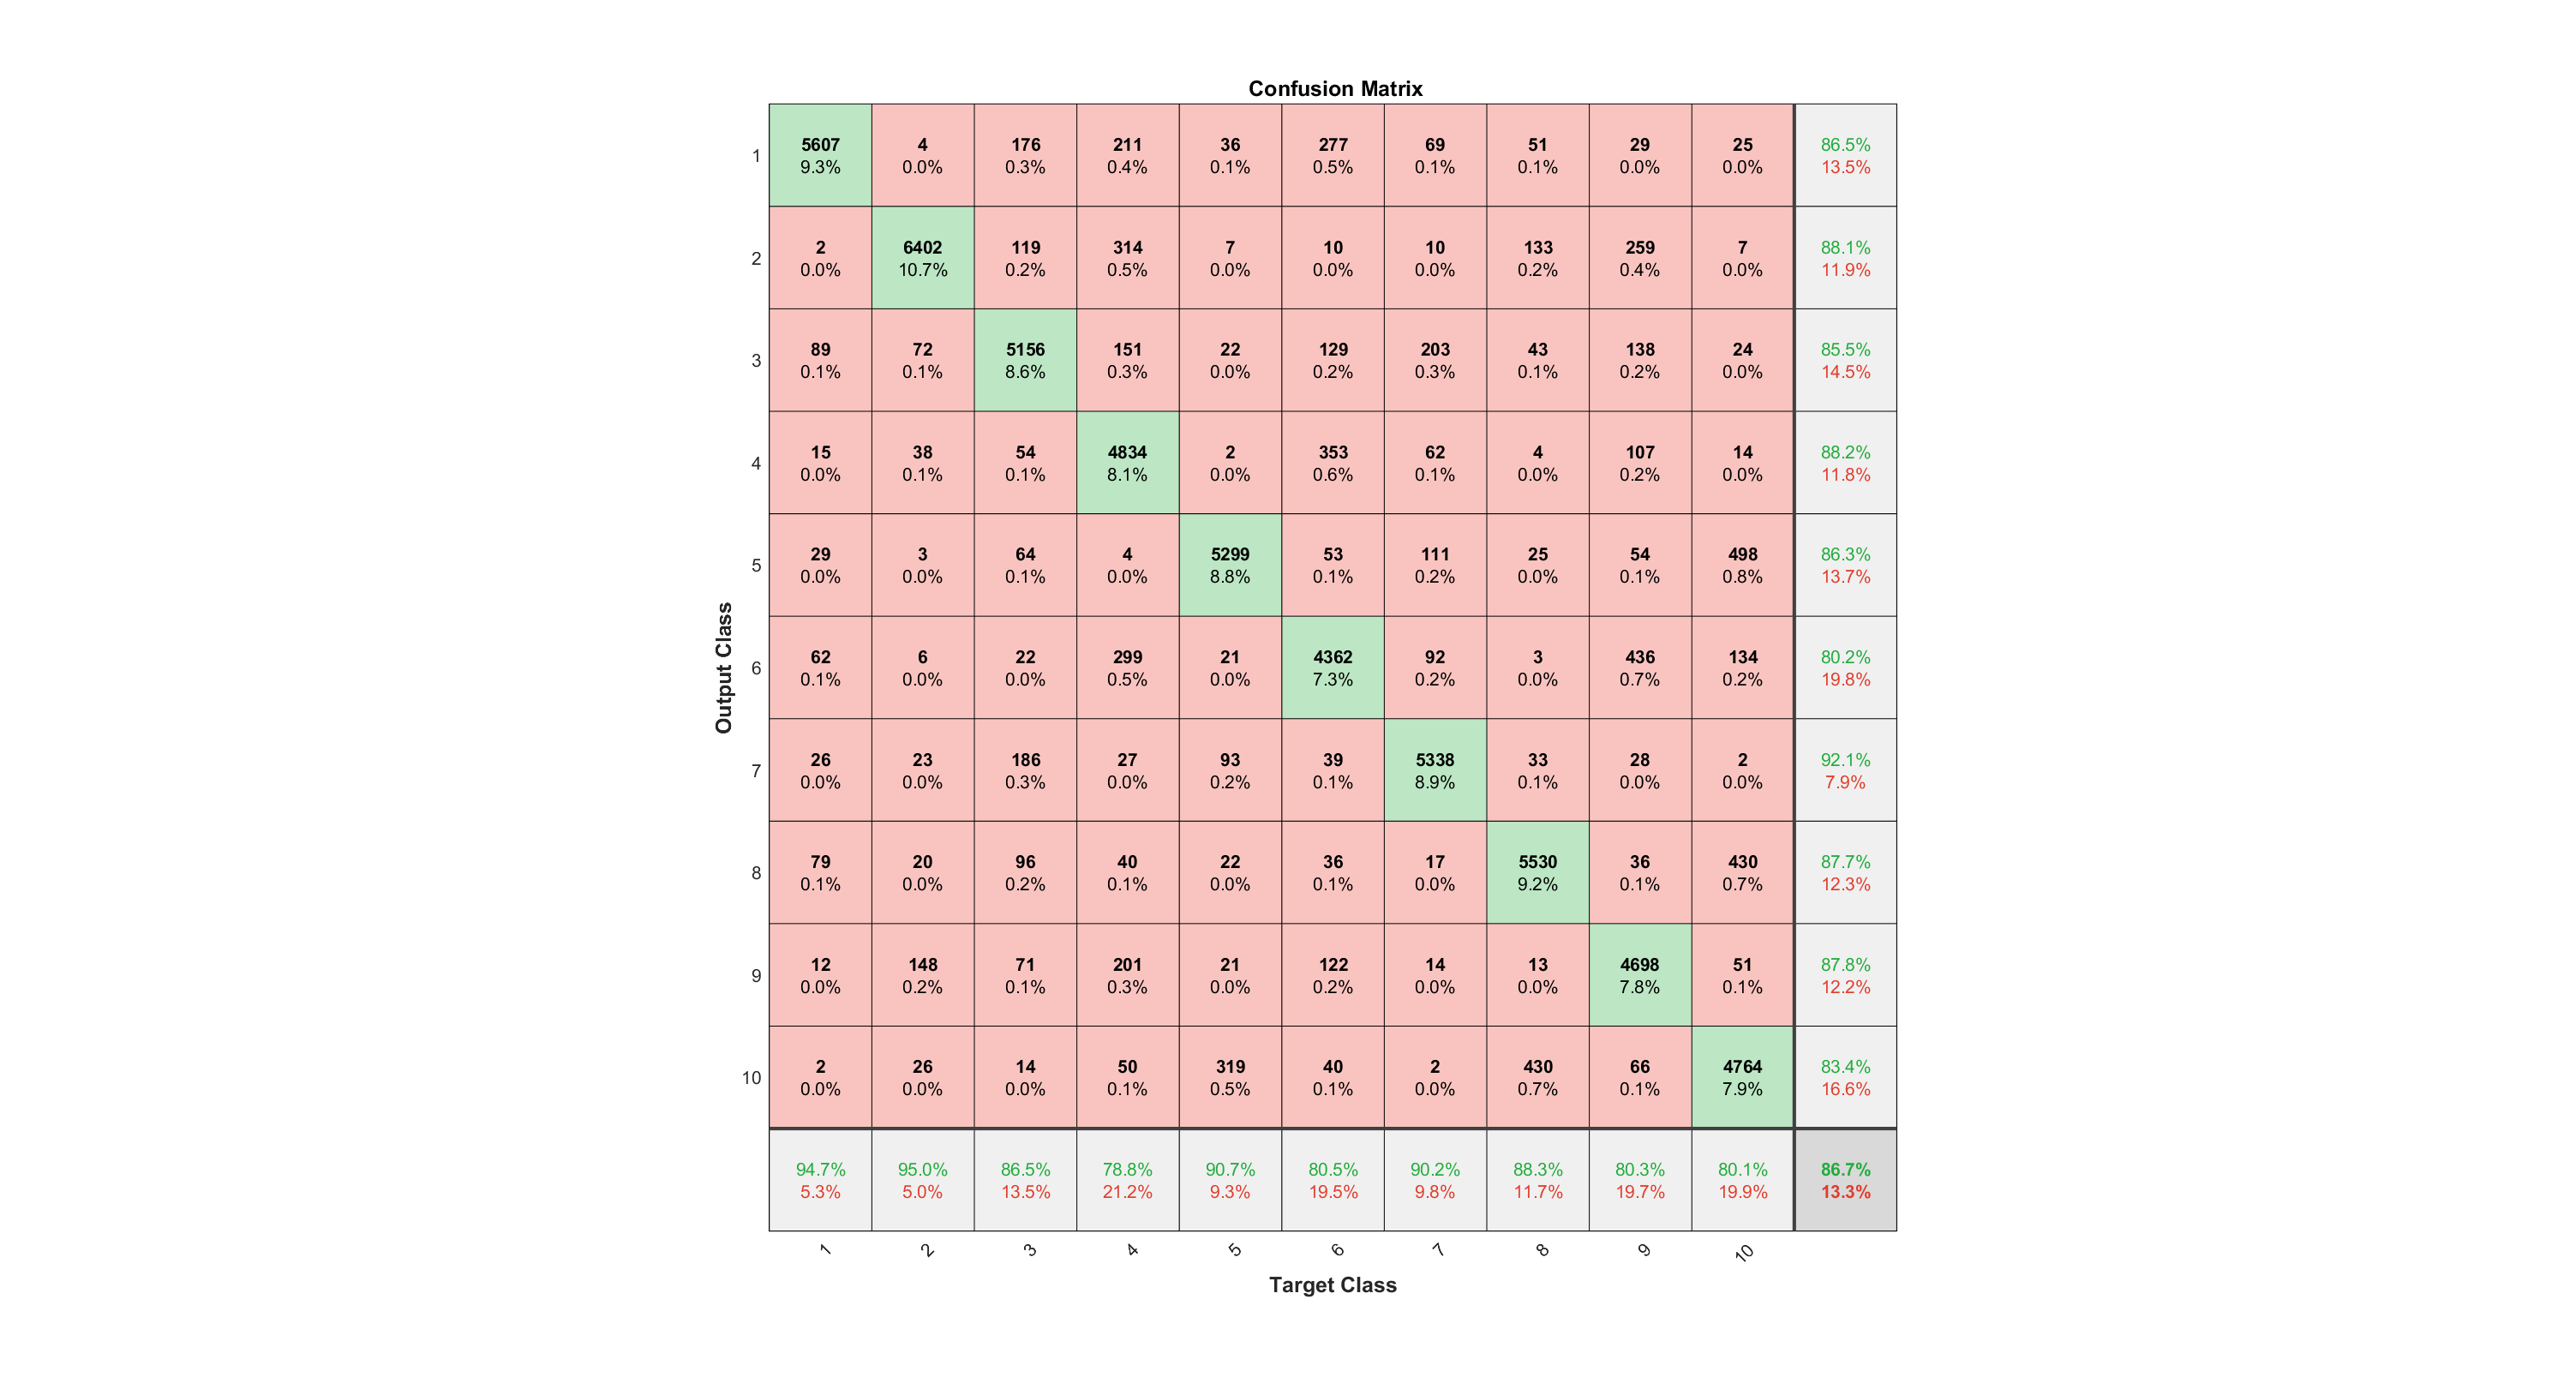
\includegraphics[width = 1.0\linewidth]{src1/Confusion_5.png}
            \caption{Confusion matrix with 5 hidden nodes}
        \end{figure}
        \begin{figure}[H]
            \centering
            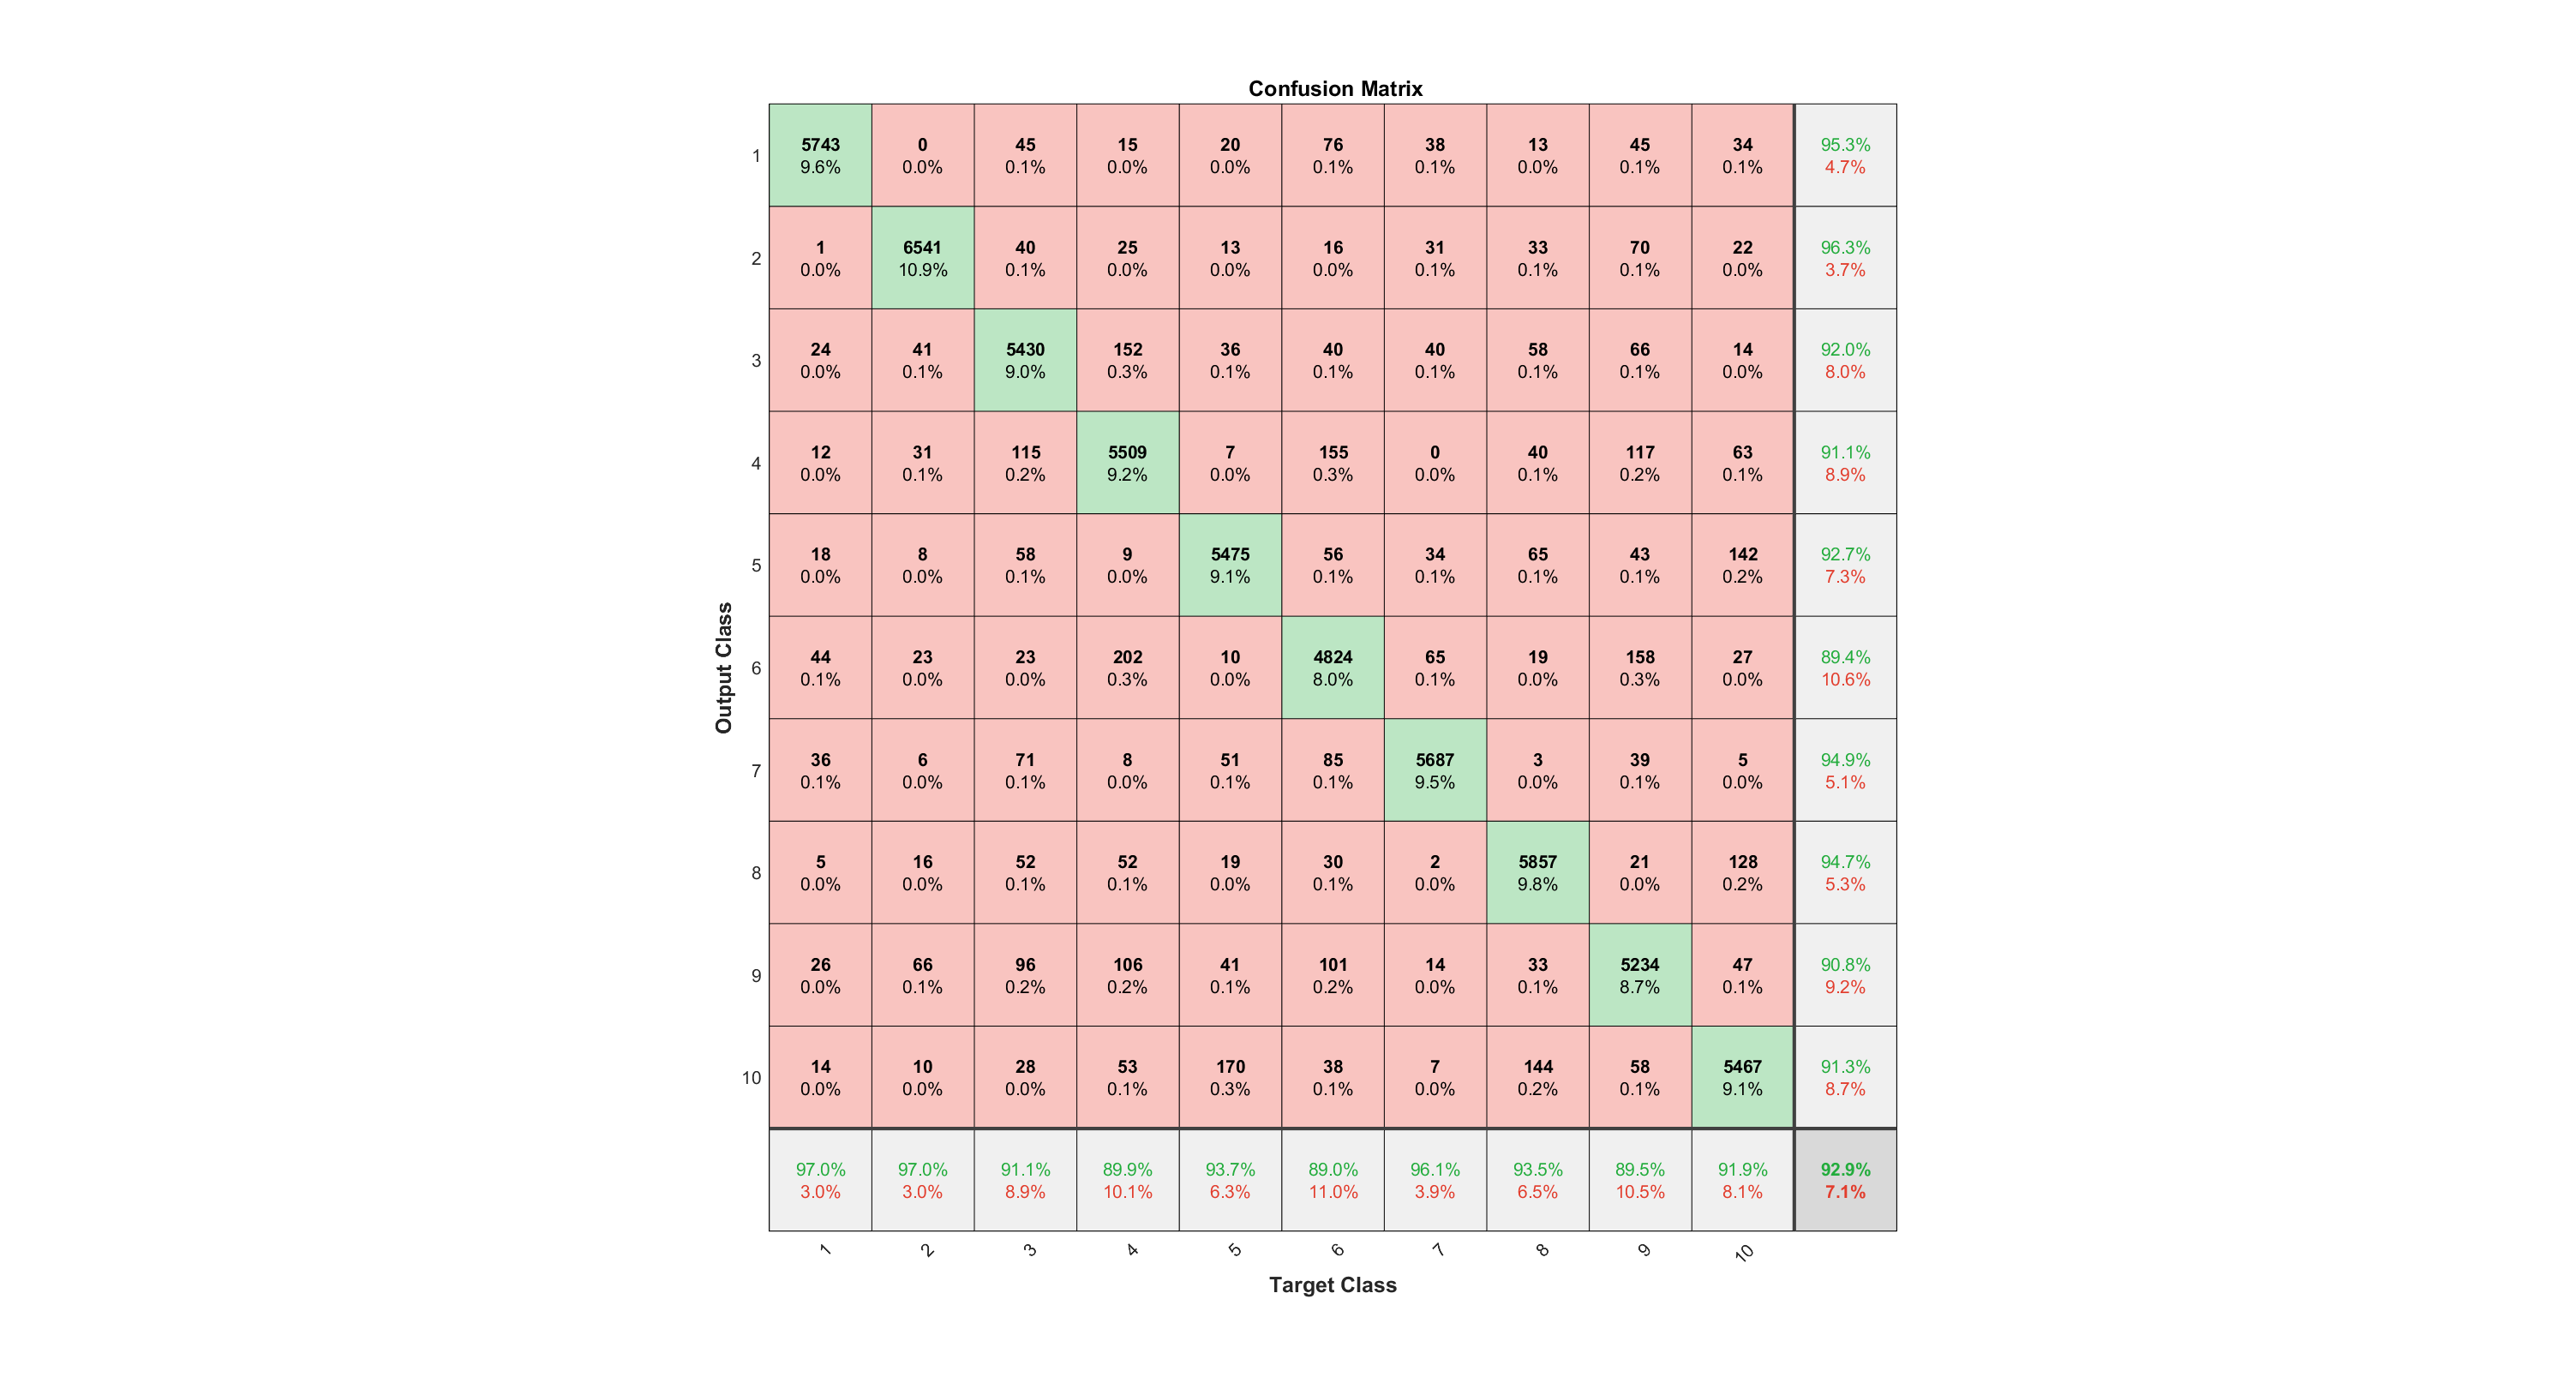
\includegraphics[width = 1.0\linewidth]{src1/Confusion_10.png}
            \caption{Confusion matrix with 10 hidden nodes}
        \end{figure}
        \begin{figure}[H]
            \centering
            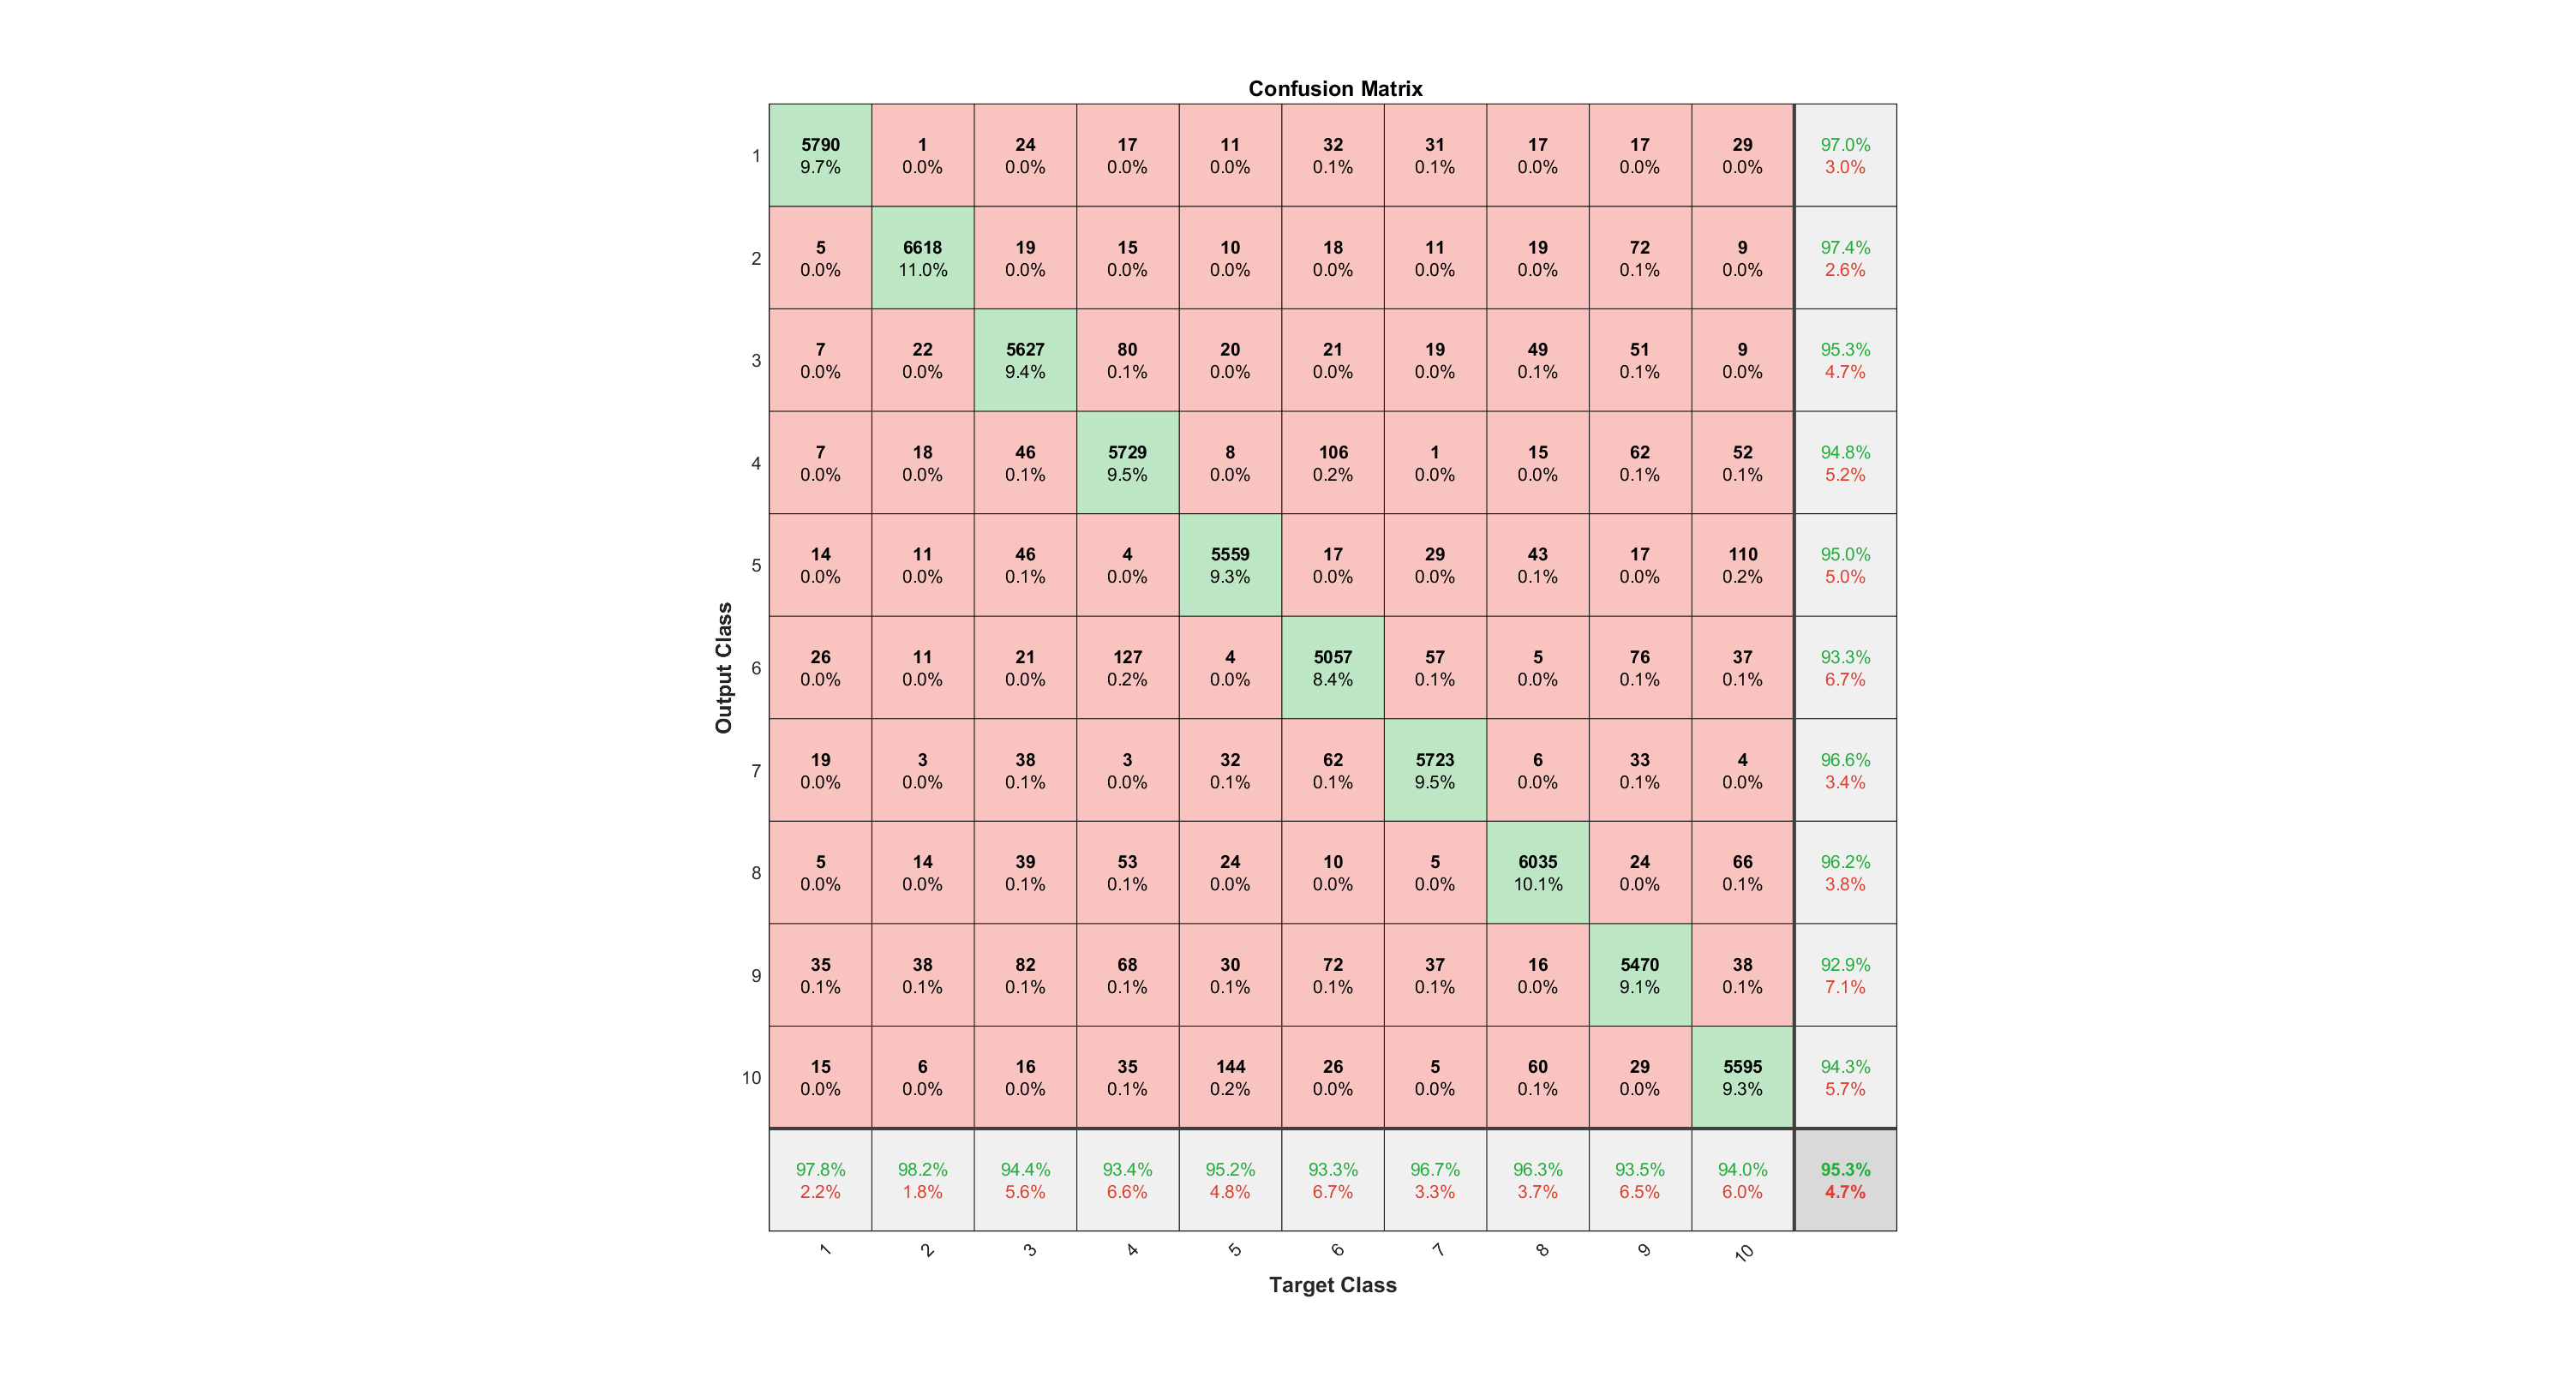
\includegraphics[width = 1.0\linewidth]{src1/Confusion_20.png}
            \caption{Confusion matrix with 20 hidden nodes}
        \end{figure}
        \begin{figure}[H]
            \centering
            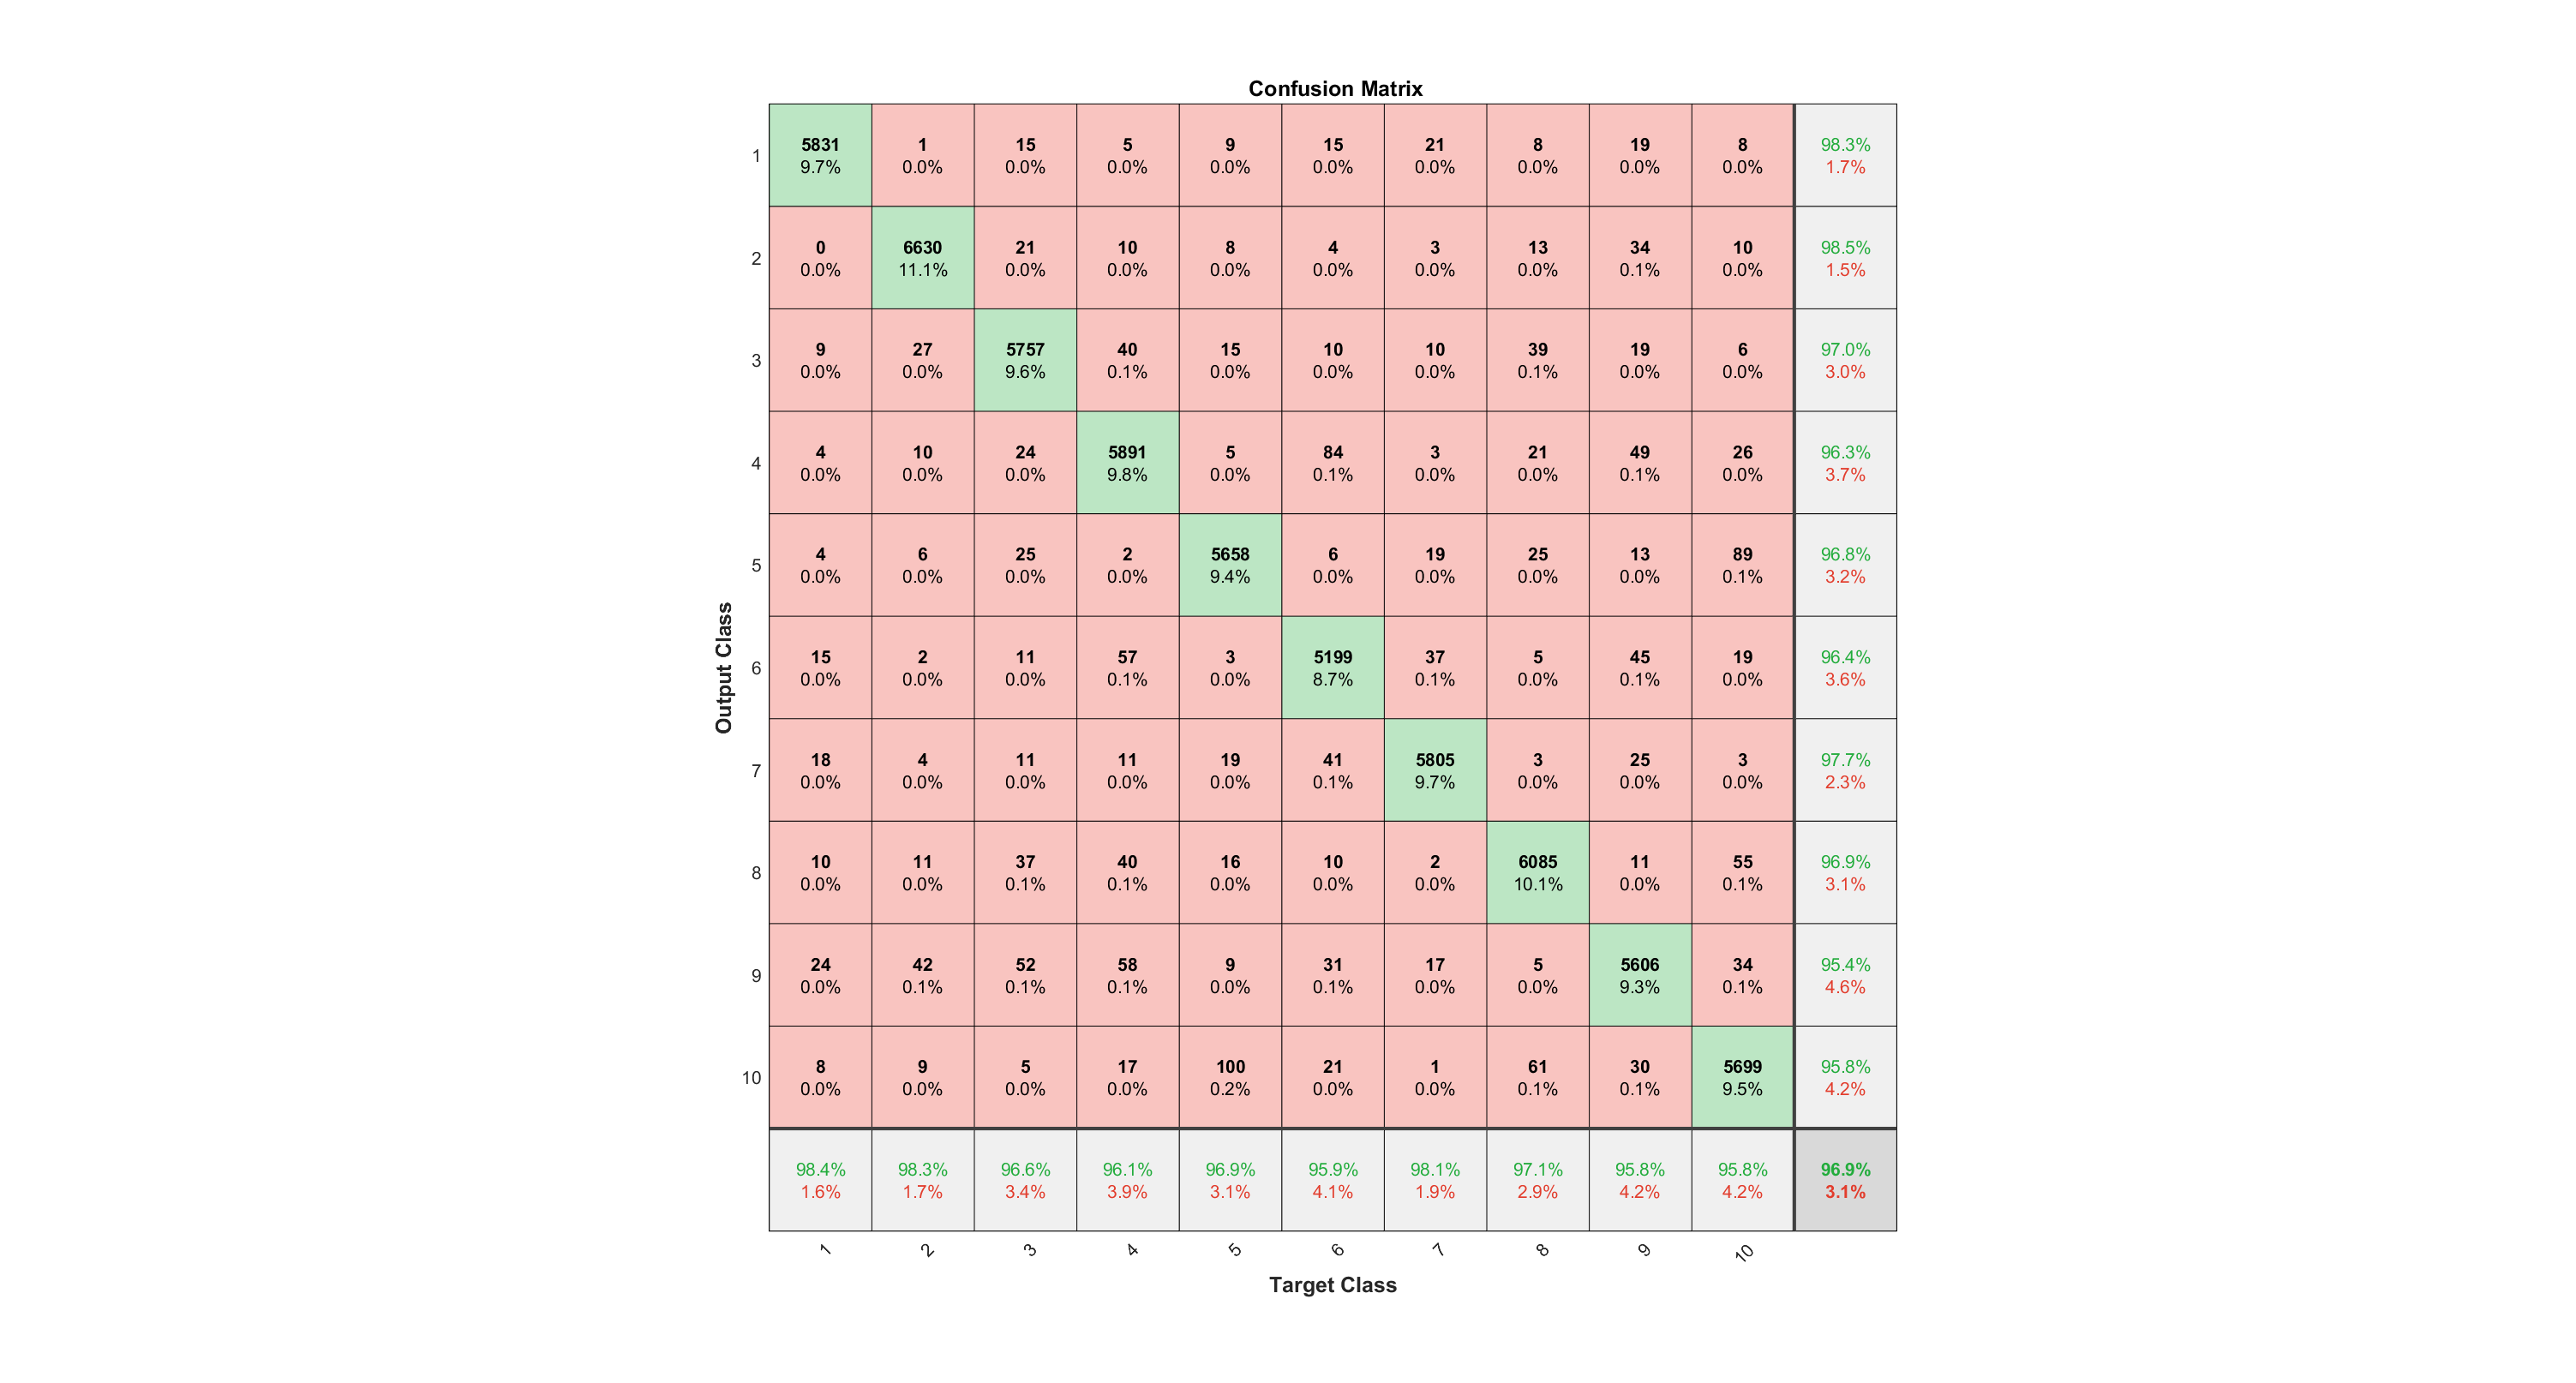
\includegraphics[width = 1.0\linewidth]{src1/Confusion_40.png}
            \caption{Confusion matrix with 40 hidden nodes}
        \end{figure}
        \begin{figure}[H]
            \centering
            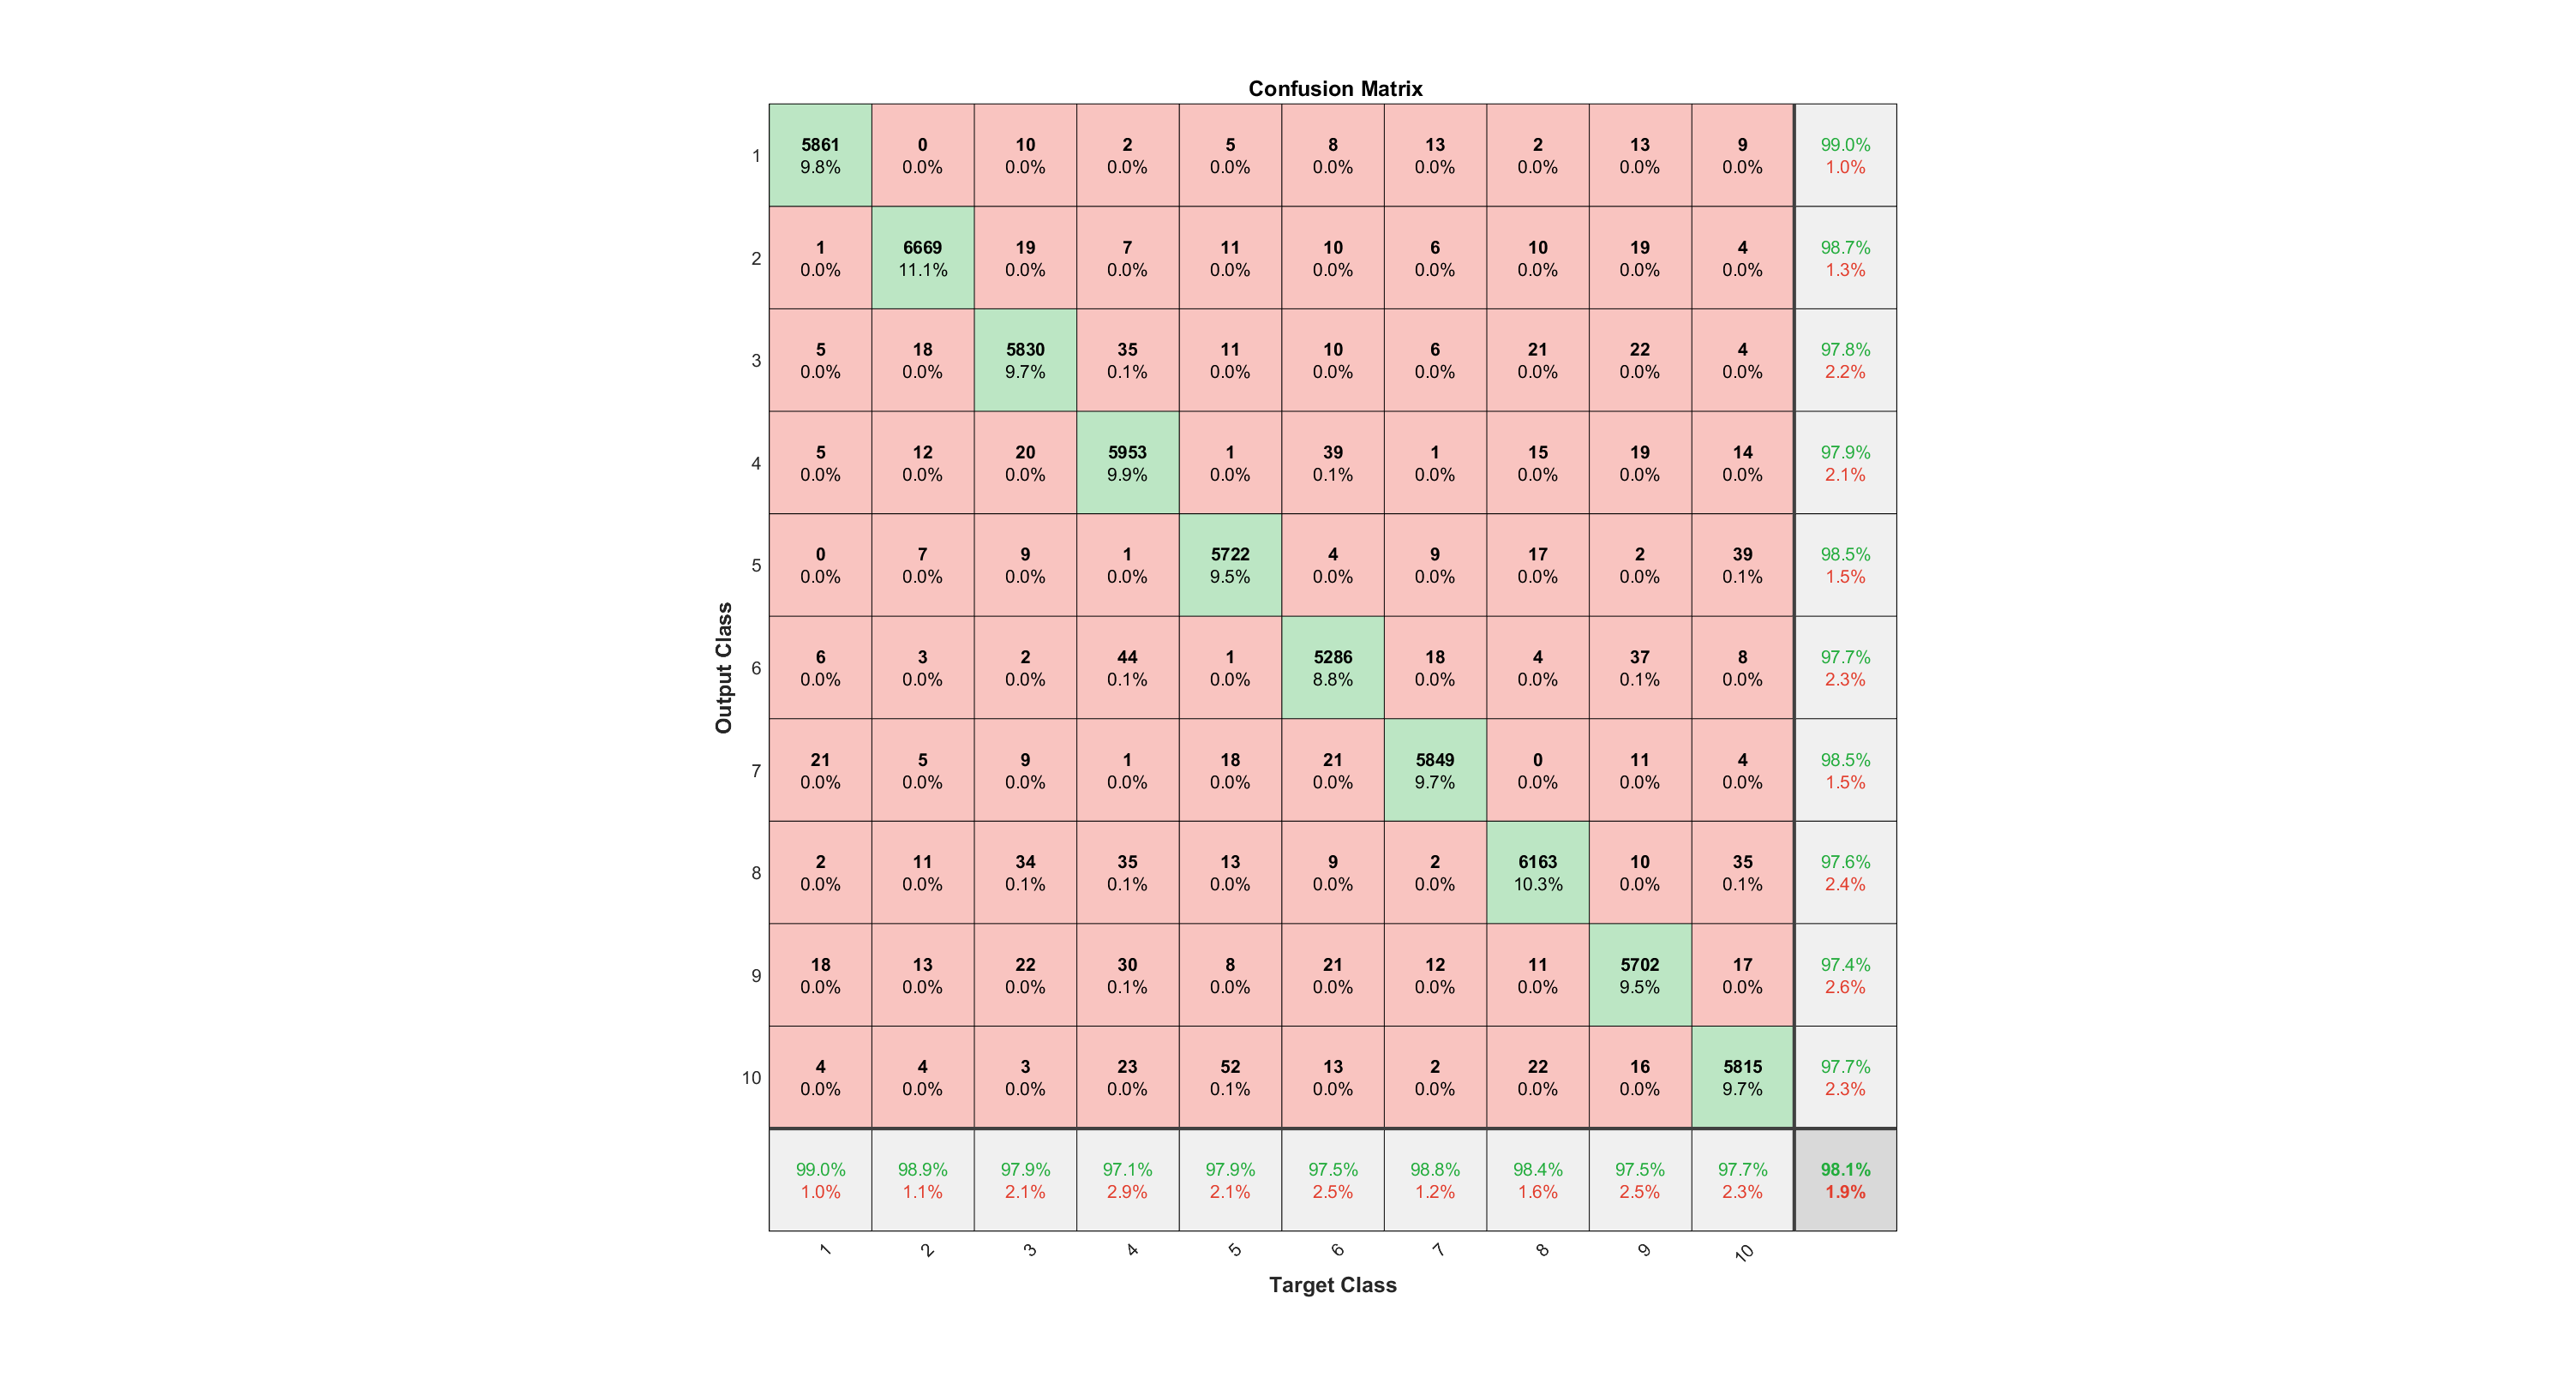
\includegraphics[width = 1.0\linewidth]{src1/Confusion_100.png}
            \caption{Confusion matrix with 100 hidden nodes}
        \end{figure}
    
        
    }

    \subsection*{Performance Curves}
    {
        \begin{figure}[H]
            \centering
            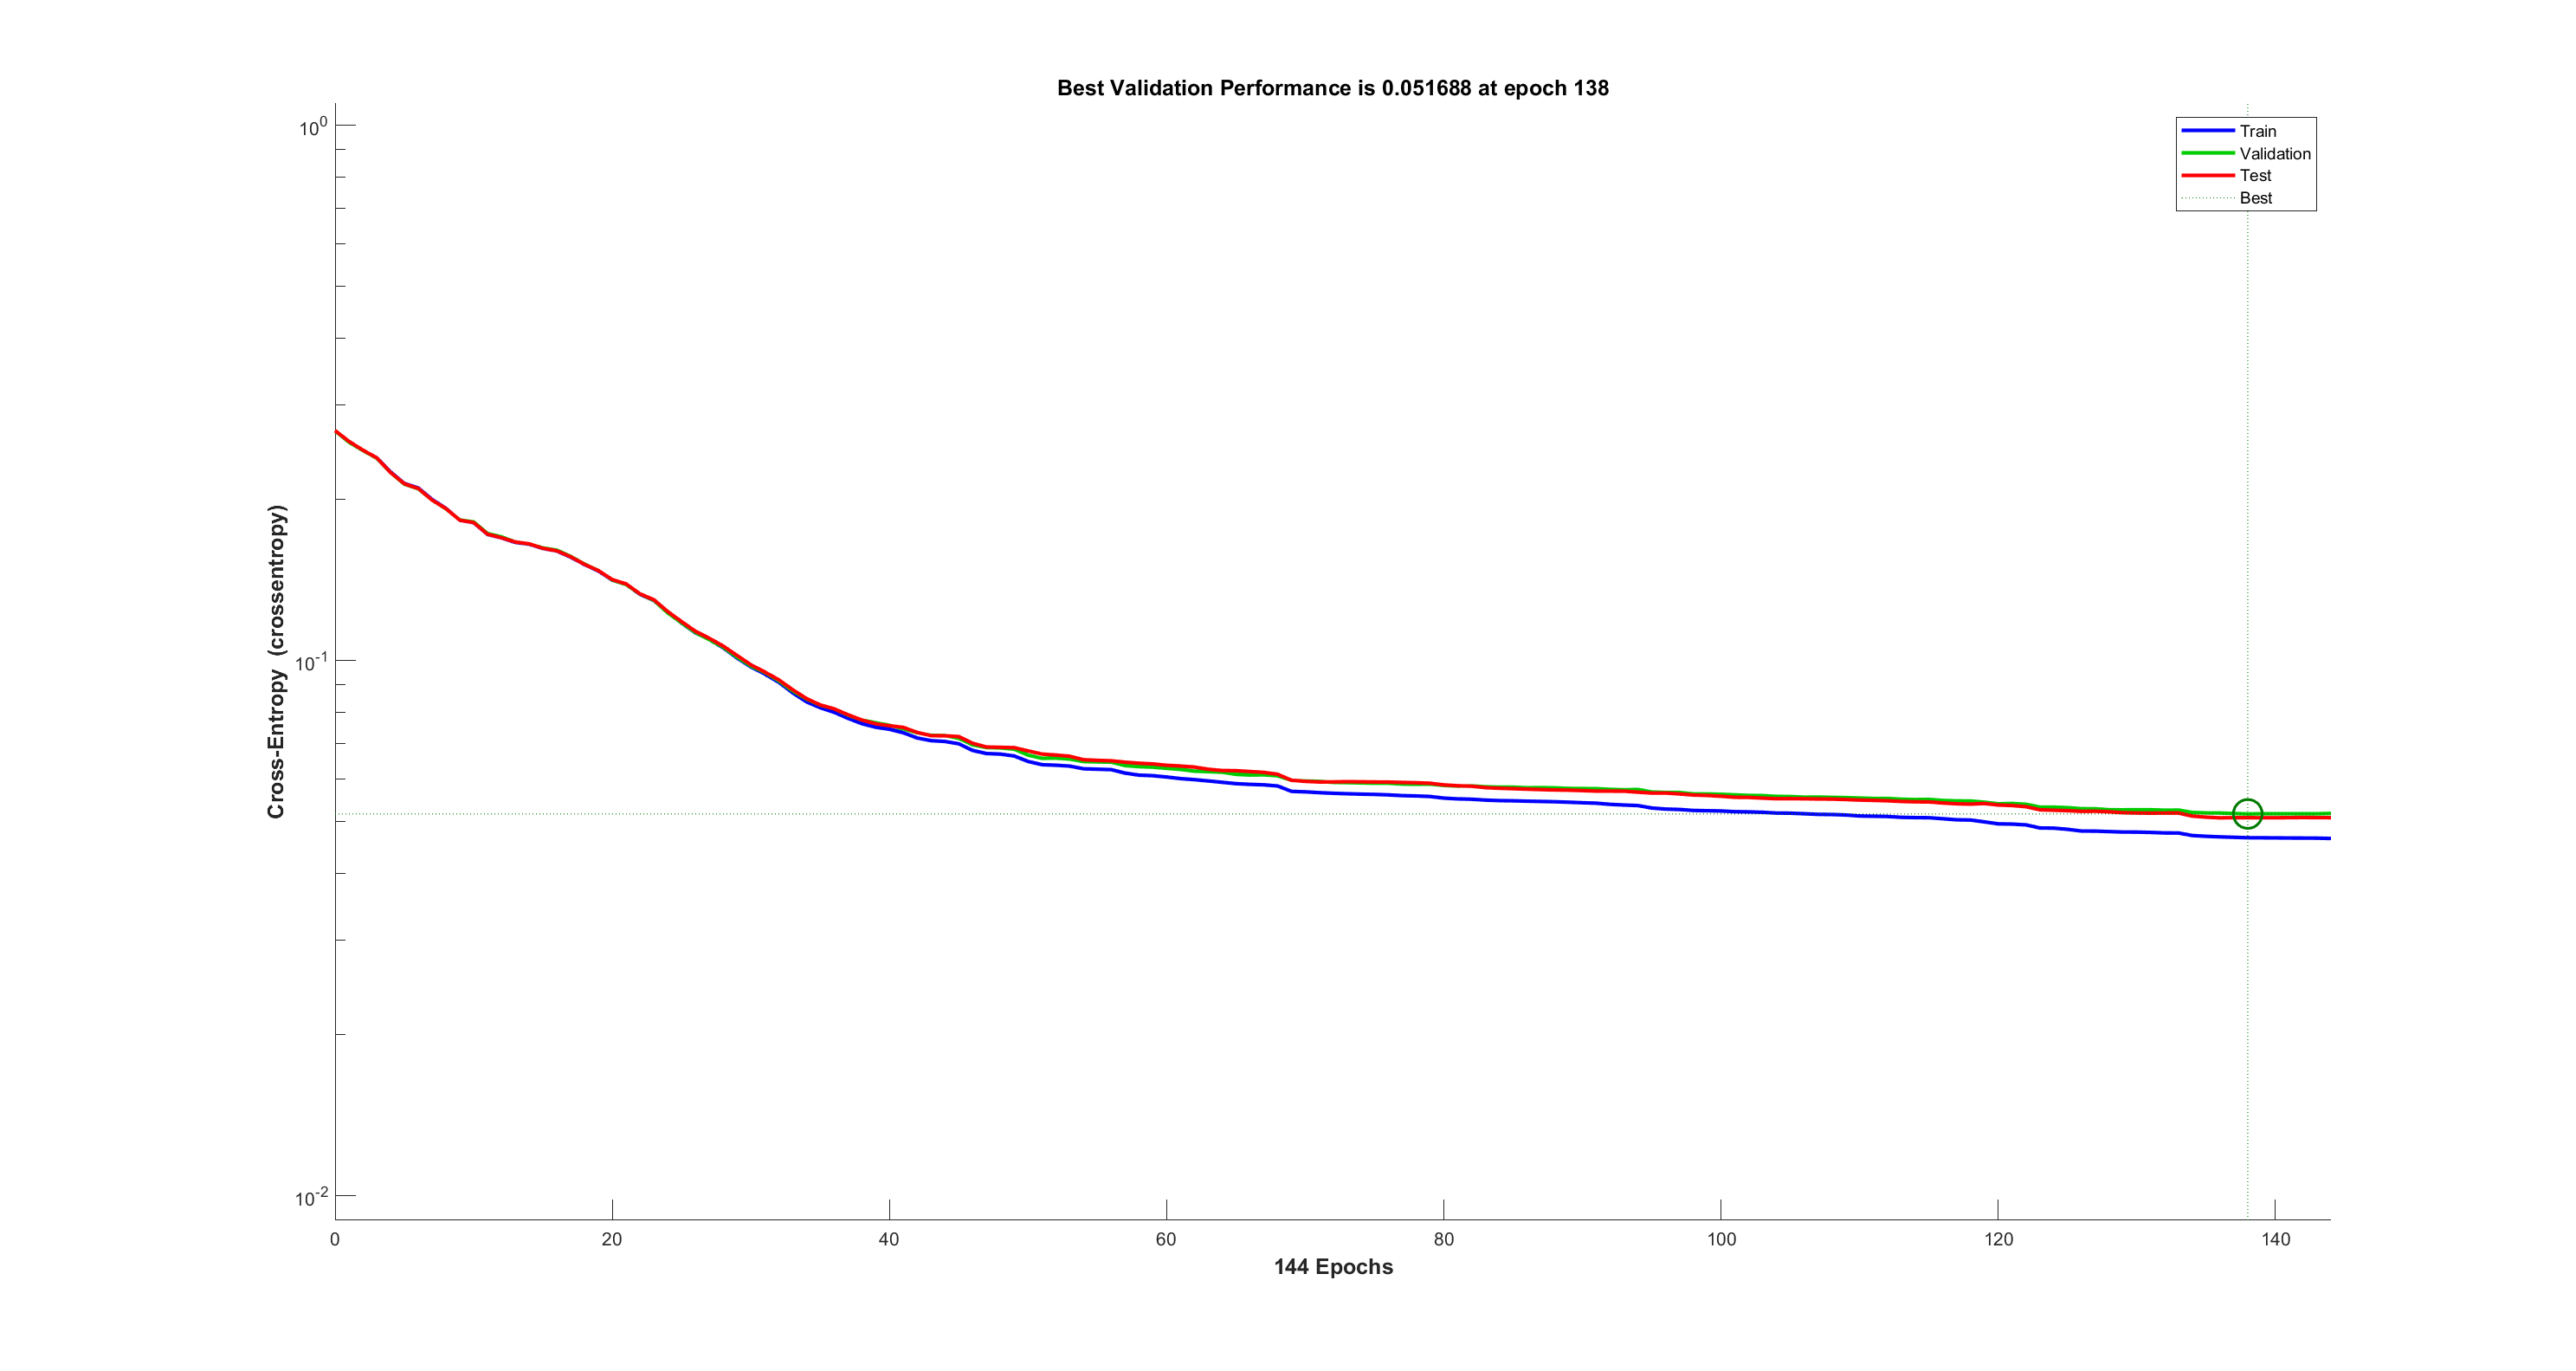
\includegraphics[width = 1.0\linewidth]{src1/Performance_5.png}
            \caption{Performance curve with 5 hidden nodes}
        \end{figure}
        \begin{figure}[H]
            \centering
            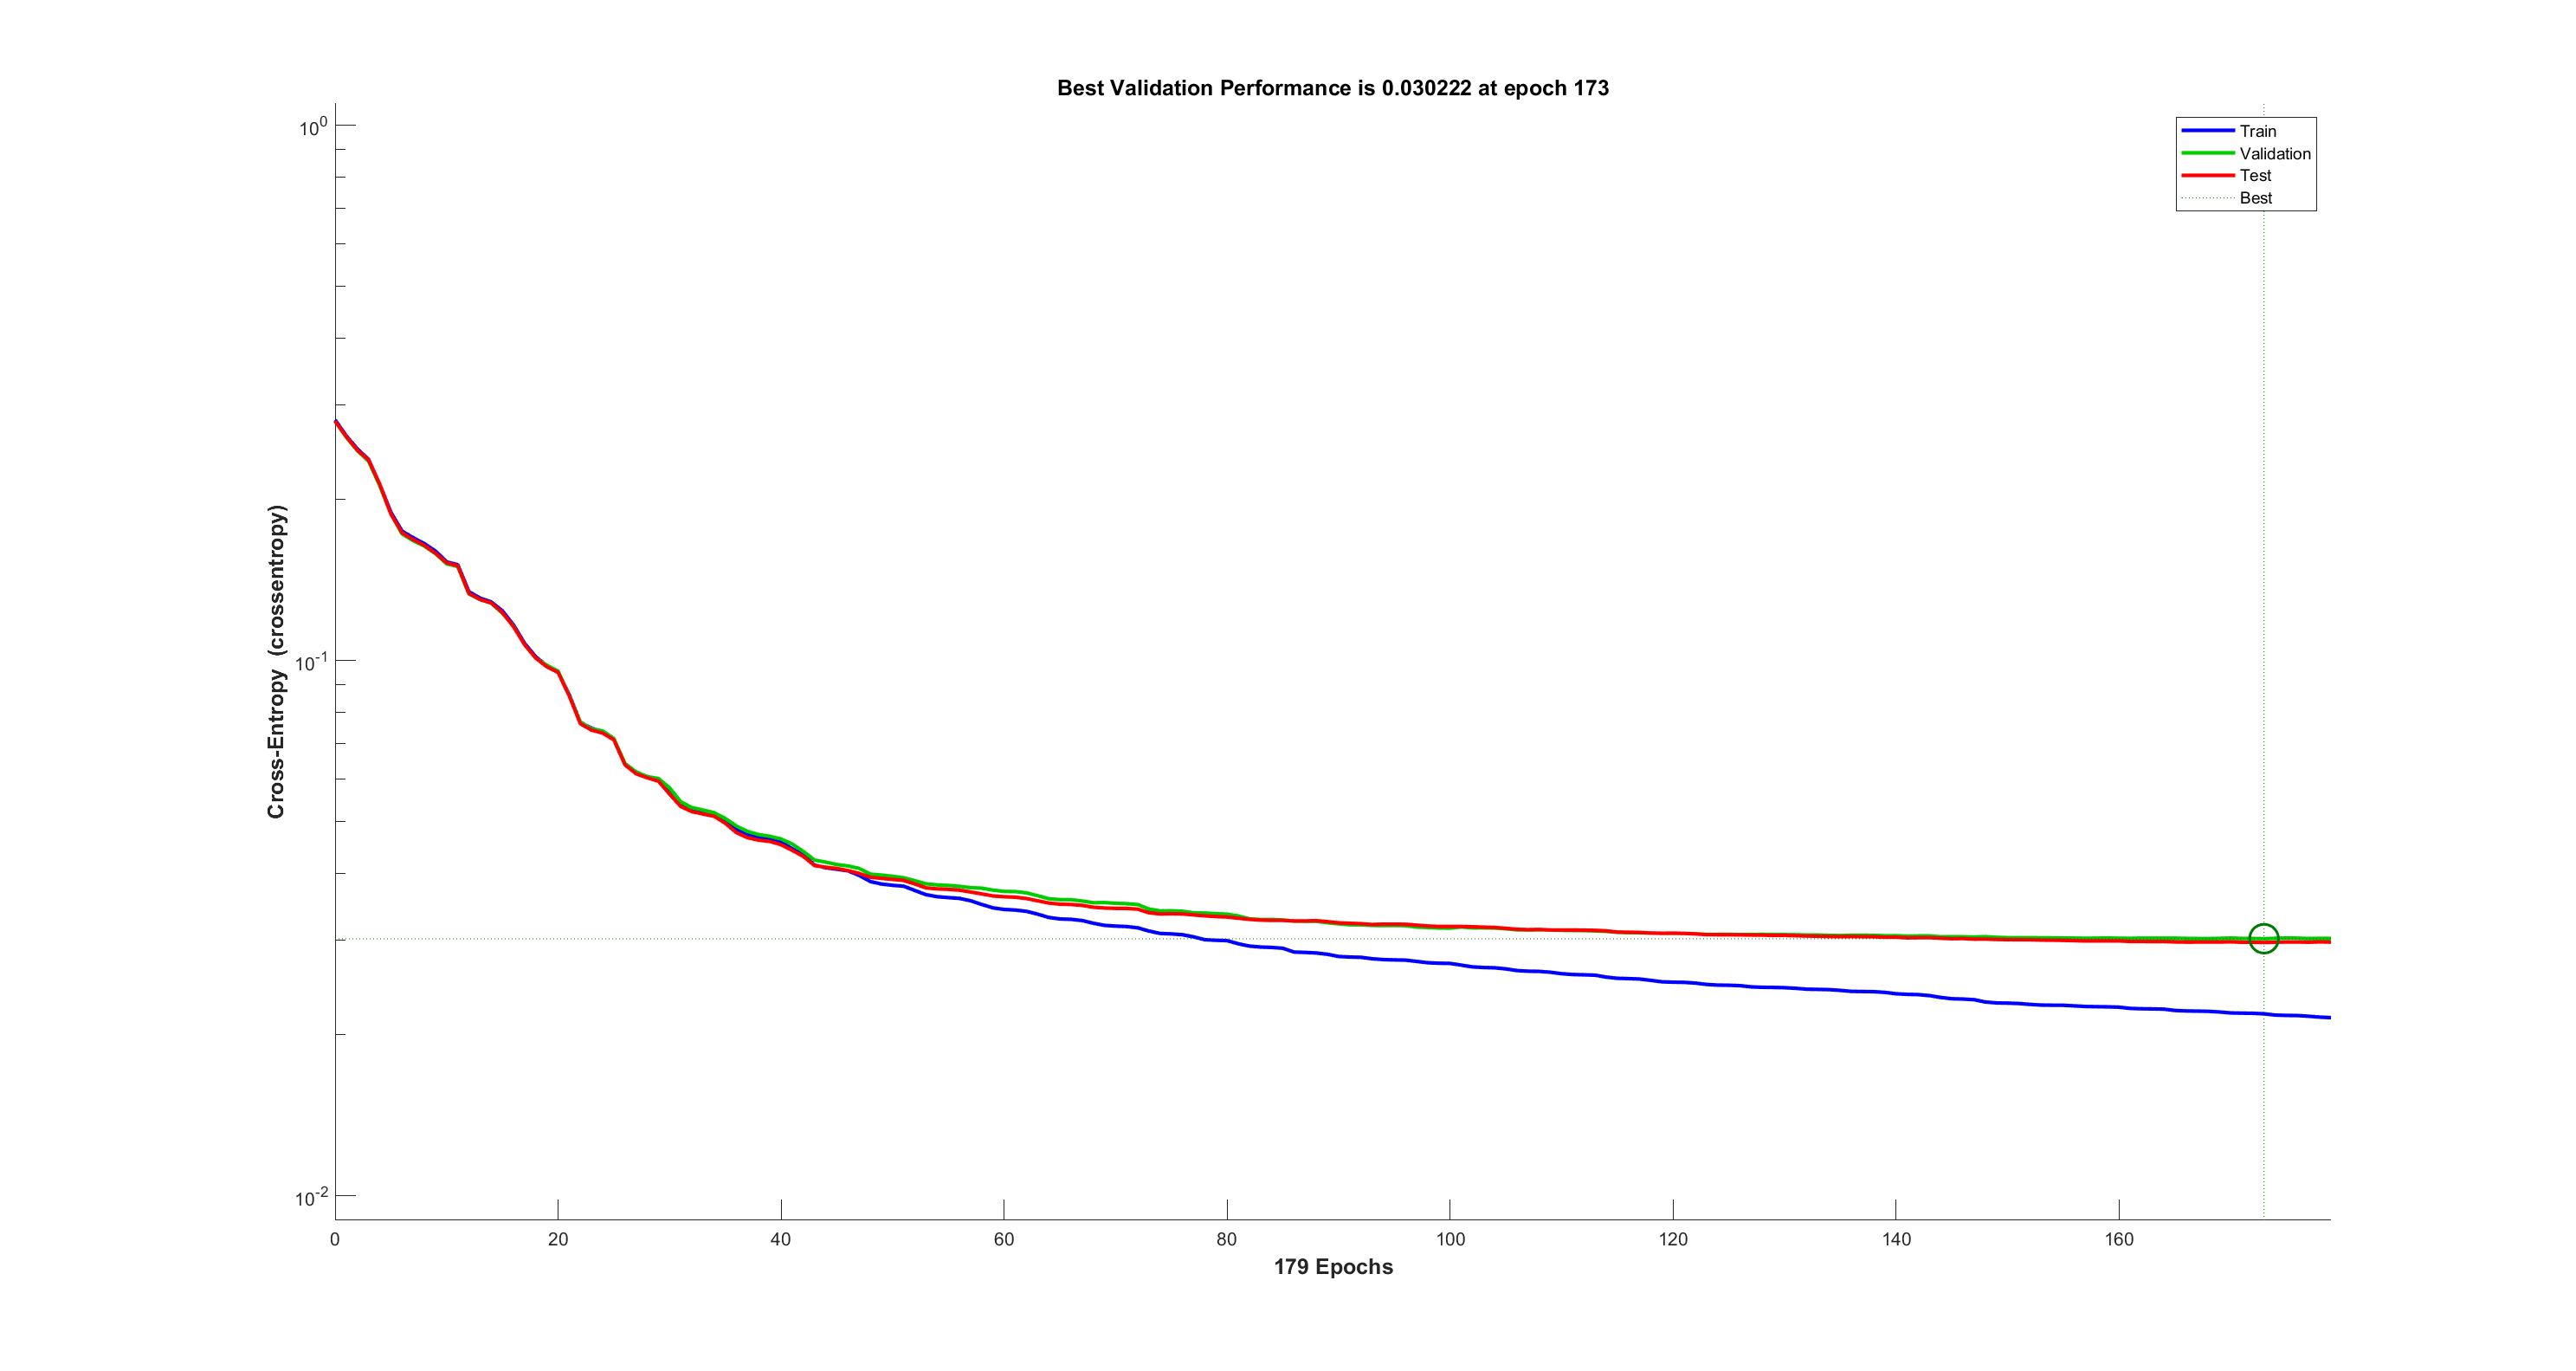
\includegraphics[width = 1.0\linewidth]{src1/Performance_10.png}
            \caption{Performance curve with 10 hidden nodes}
        \end{figure}
        \begin{figure}[H]
            \centering
            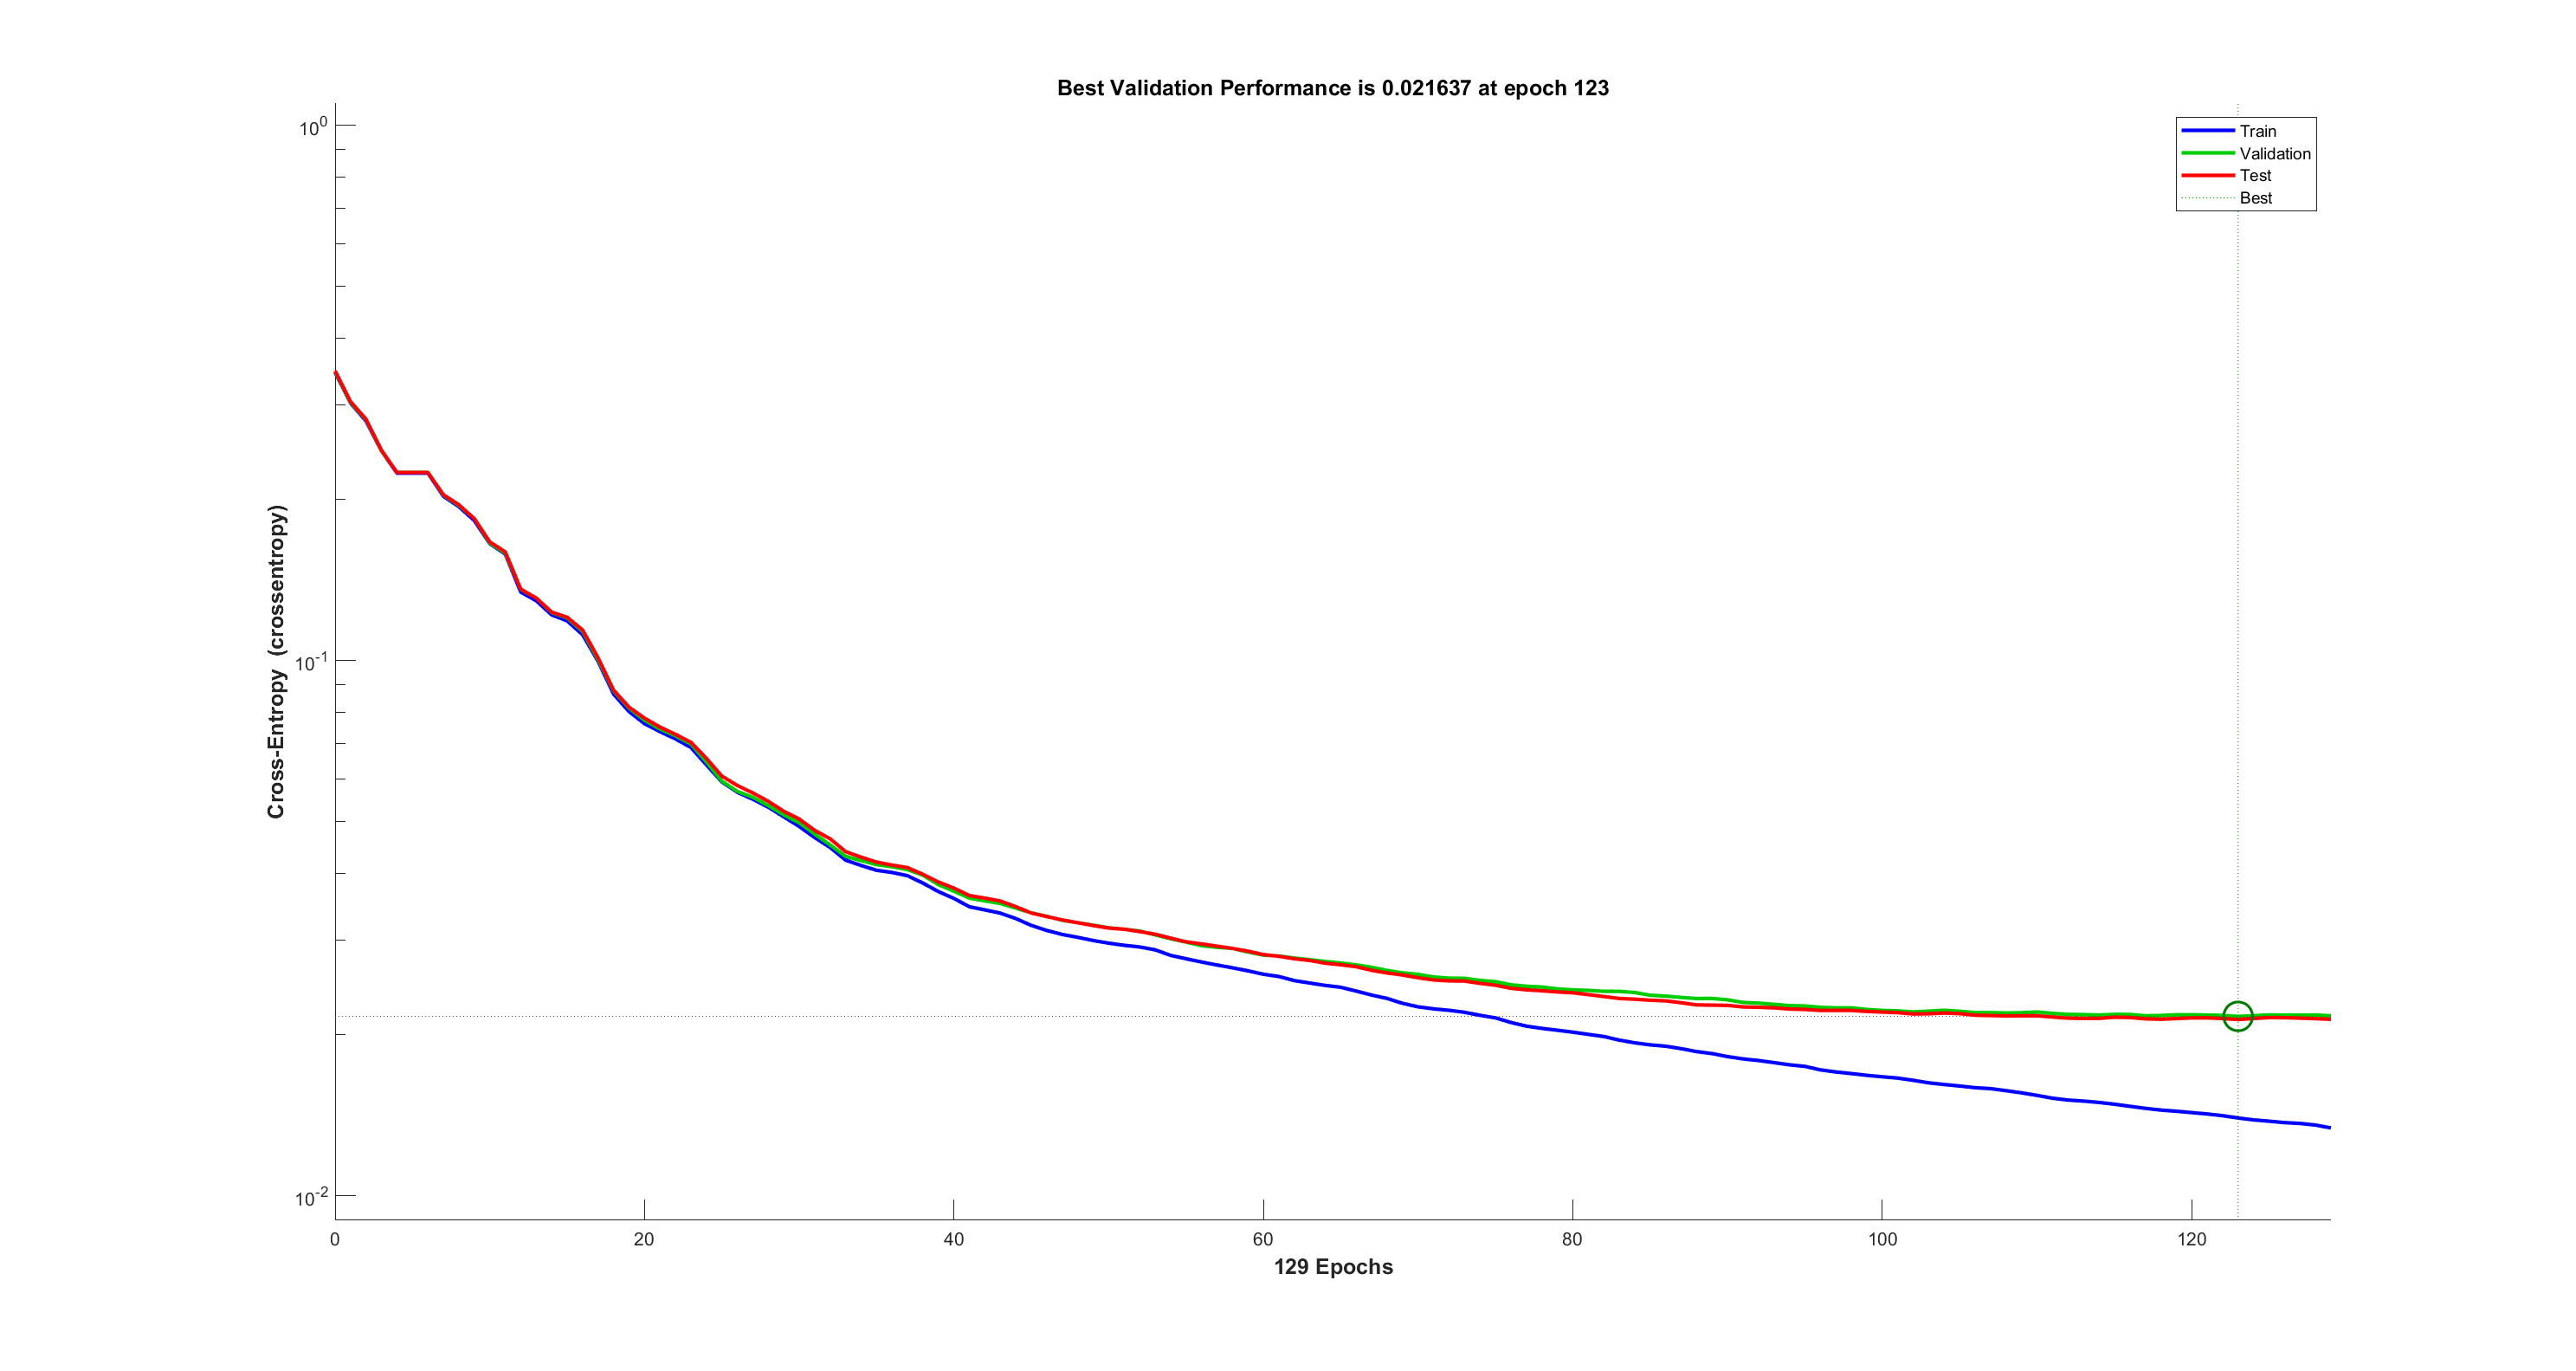
\includegraphics[width = 1.0\linewidth]{src1/Performance_20.png}
            \caption{Performance curve with 20 hidden nodes}
        \end{figure}
        \begin{figure}[H]
            \centering
            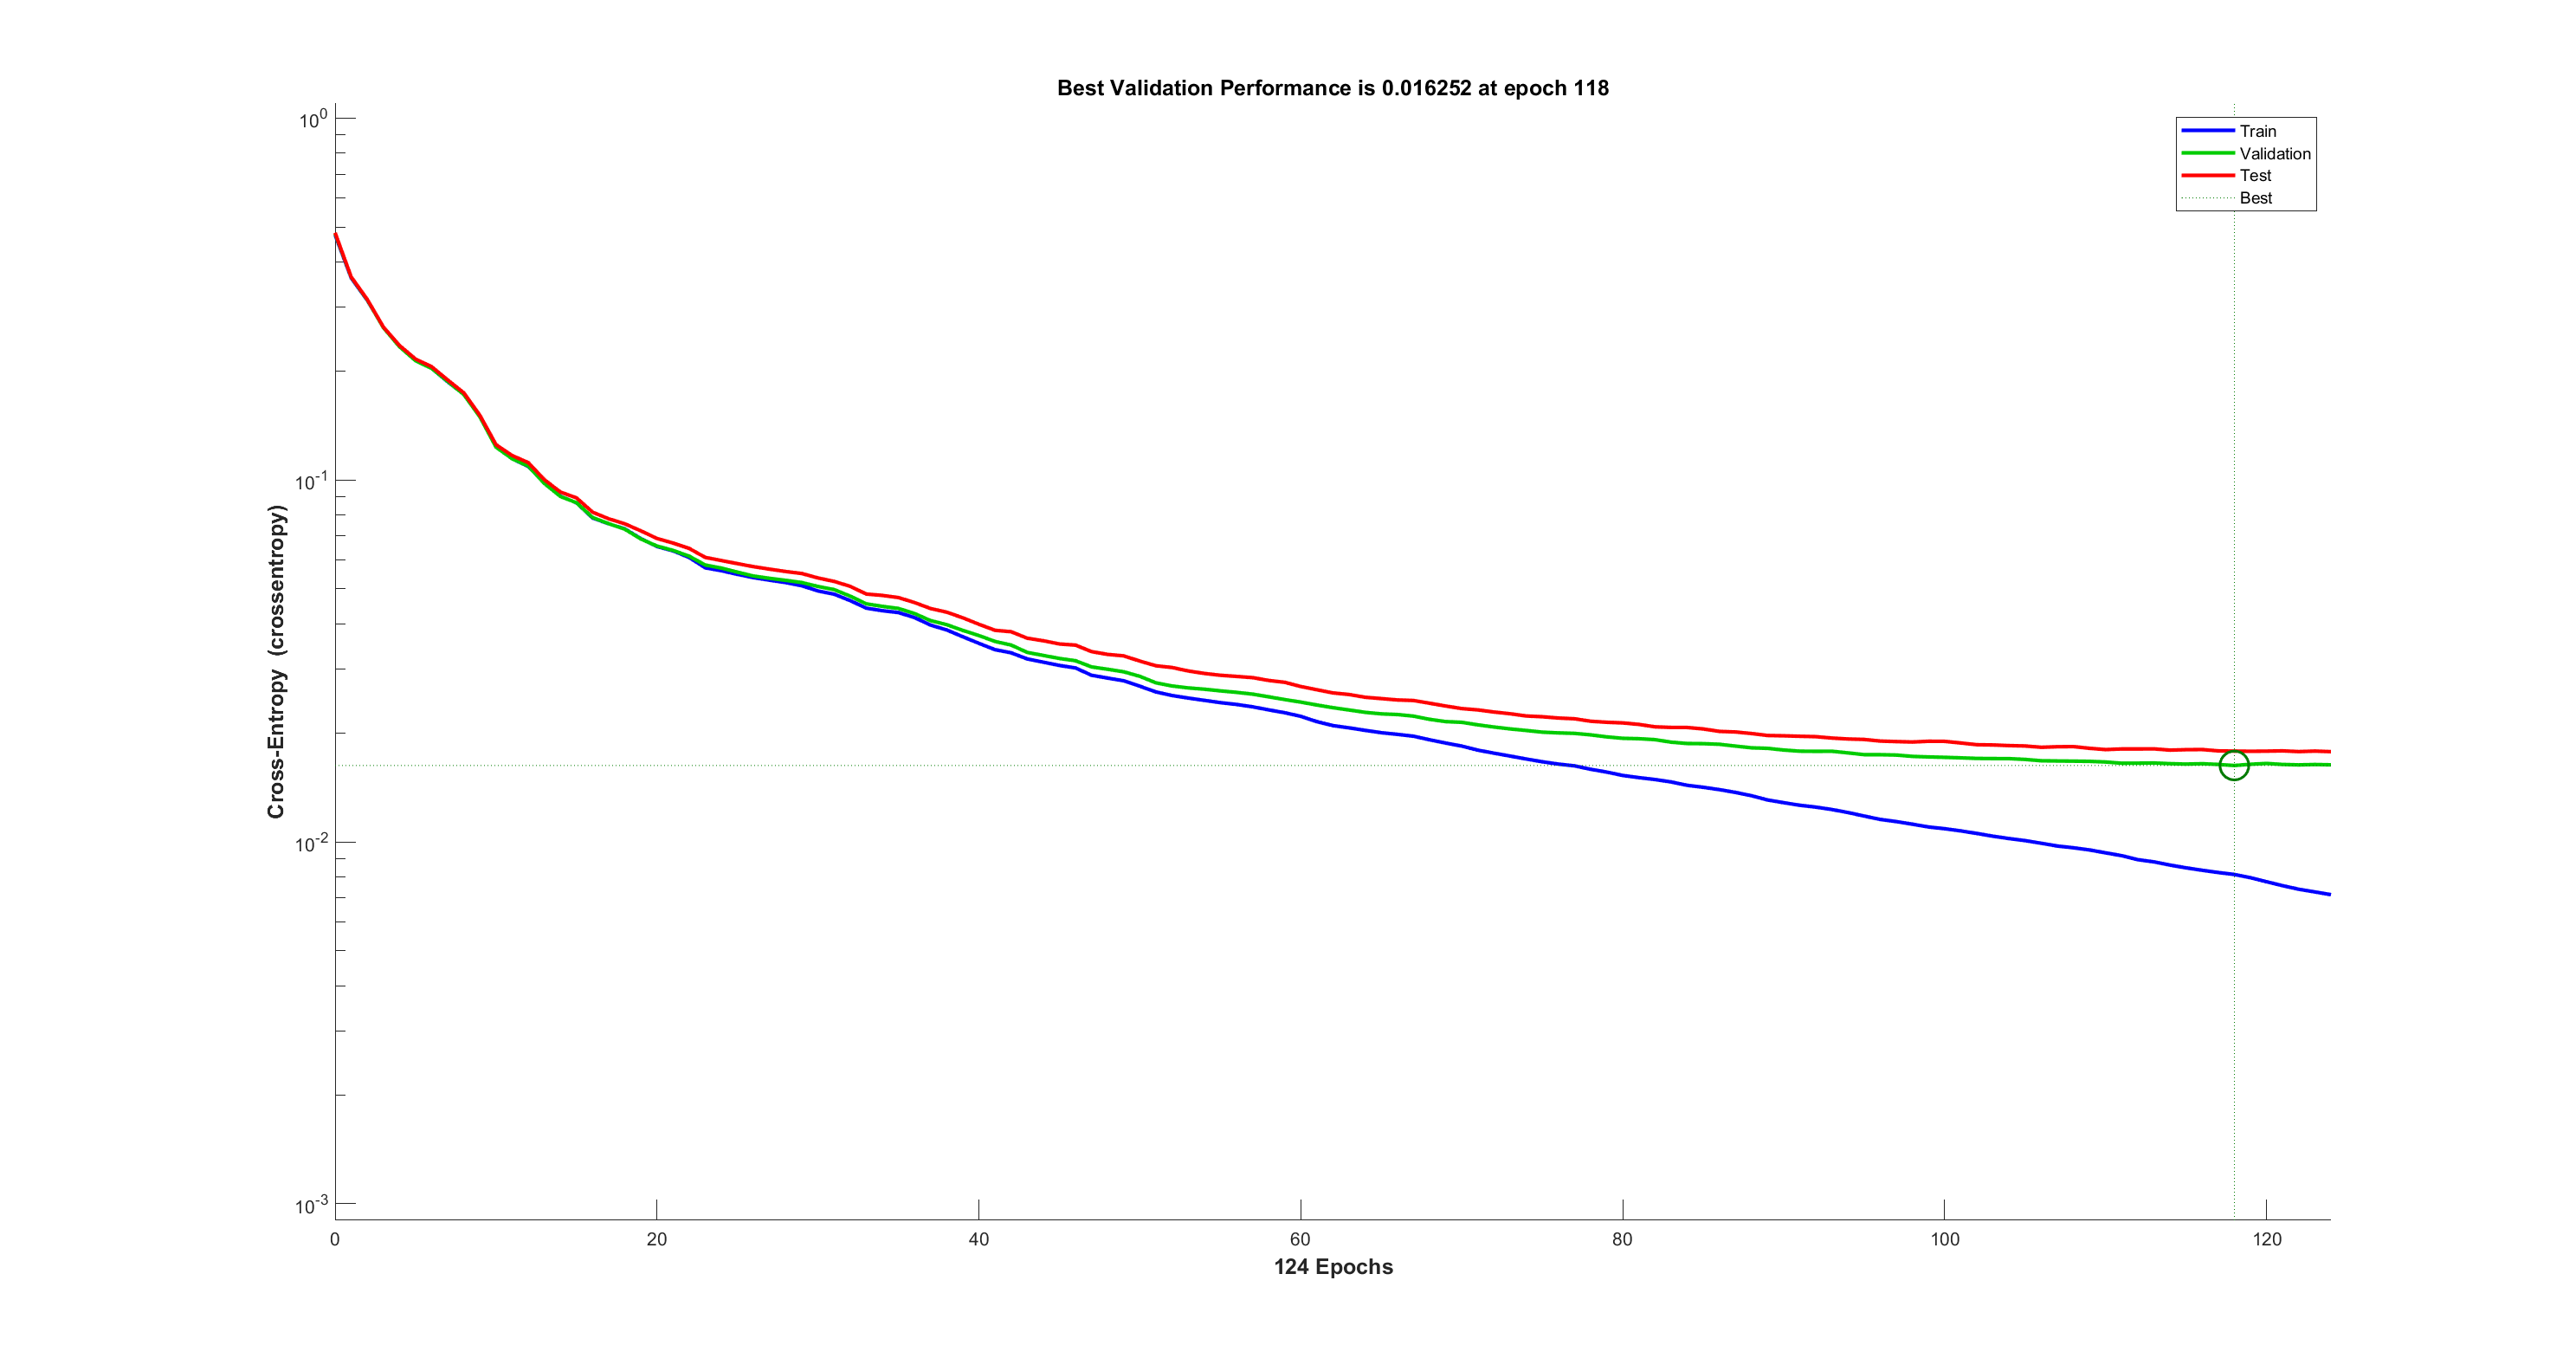
\includegraphics[width = 1.0\linewidth]{src1/Performance_40.png}
            \caption{Performance curve with 40 hidden nodes}
        \end{figure}
        \begin{figure}[H]
            \centering
            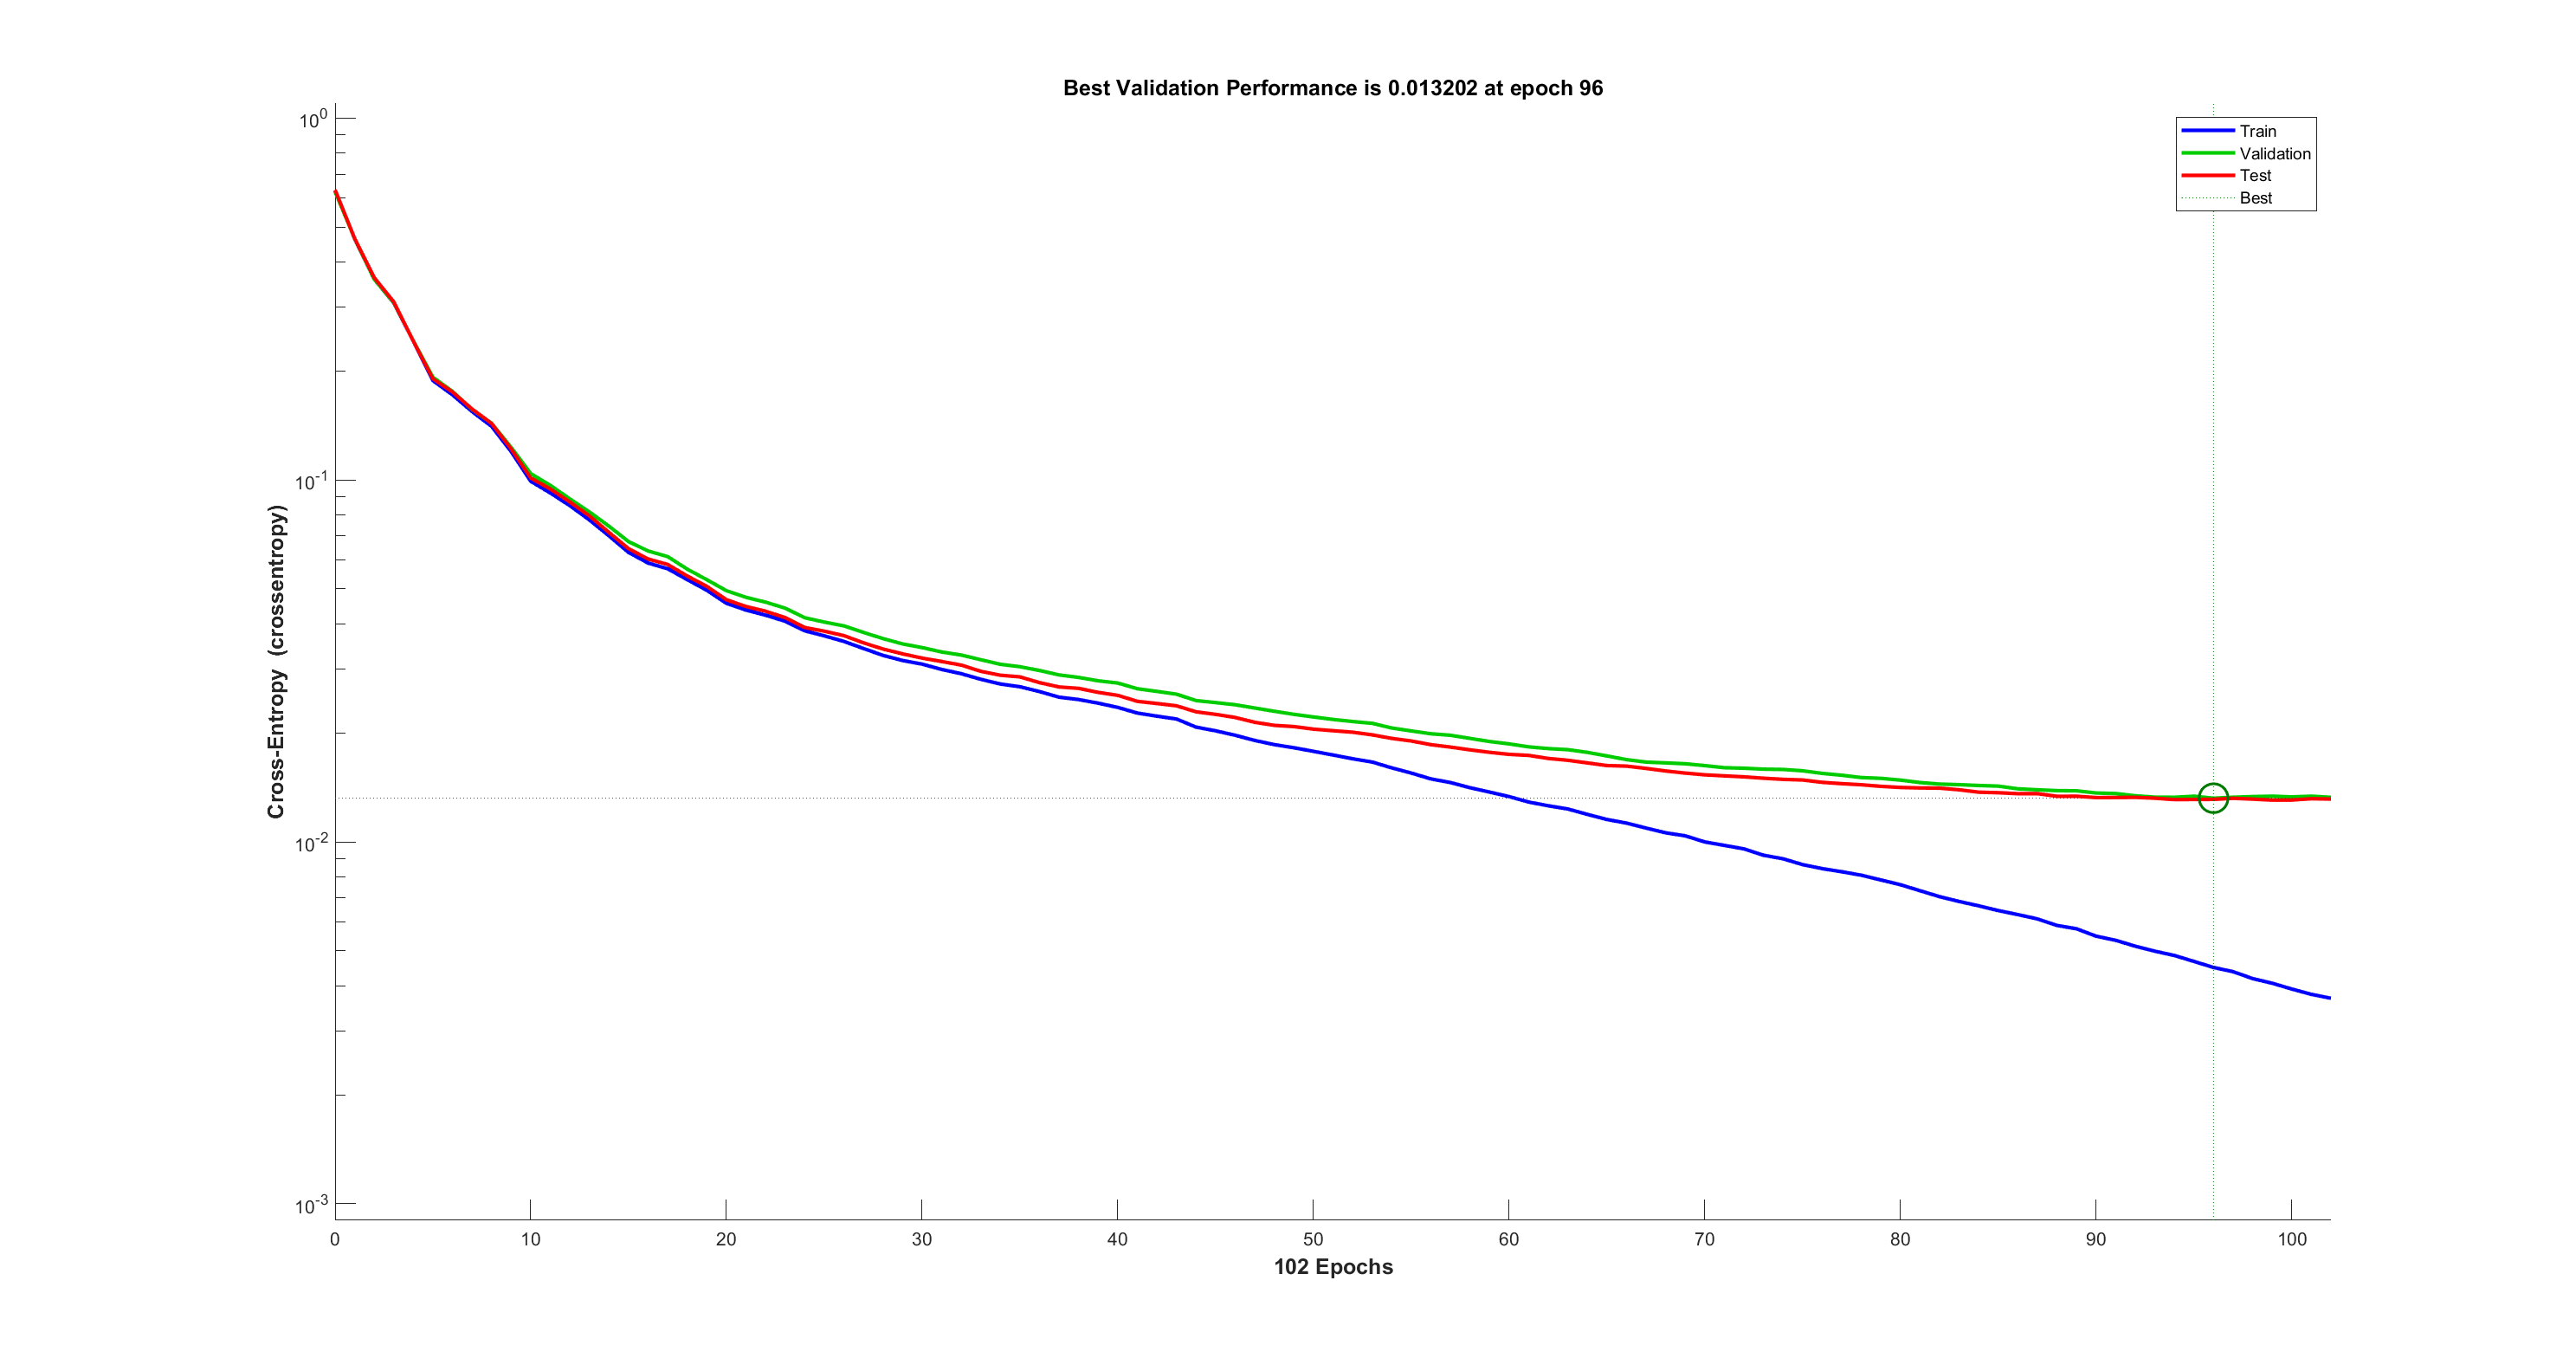
\includegraphics[width = 1.0\linewidth]{src1/Performance_100.png}
            \caption{Performance curve with 100 hidden nodes}
        \end{figure}
    }

    \subsection*{Plots of Rate of Correctness (ROC)}
    {
        \begin{figure}[H]
            \centering
            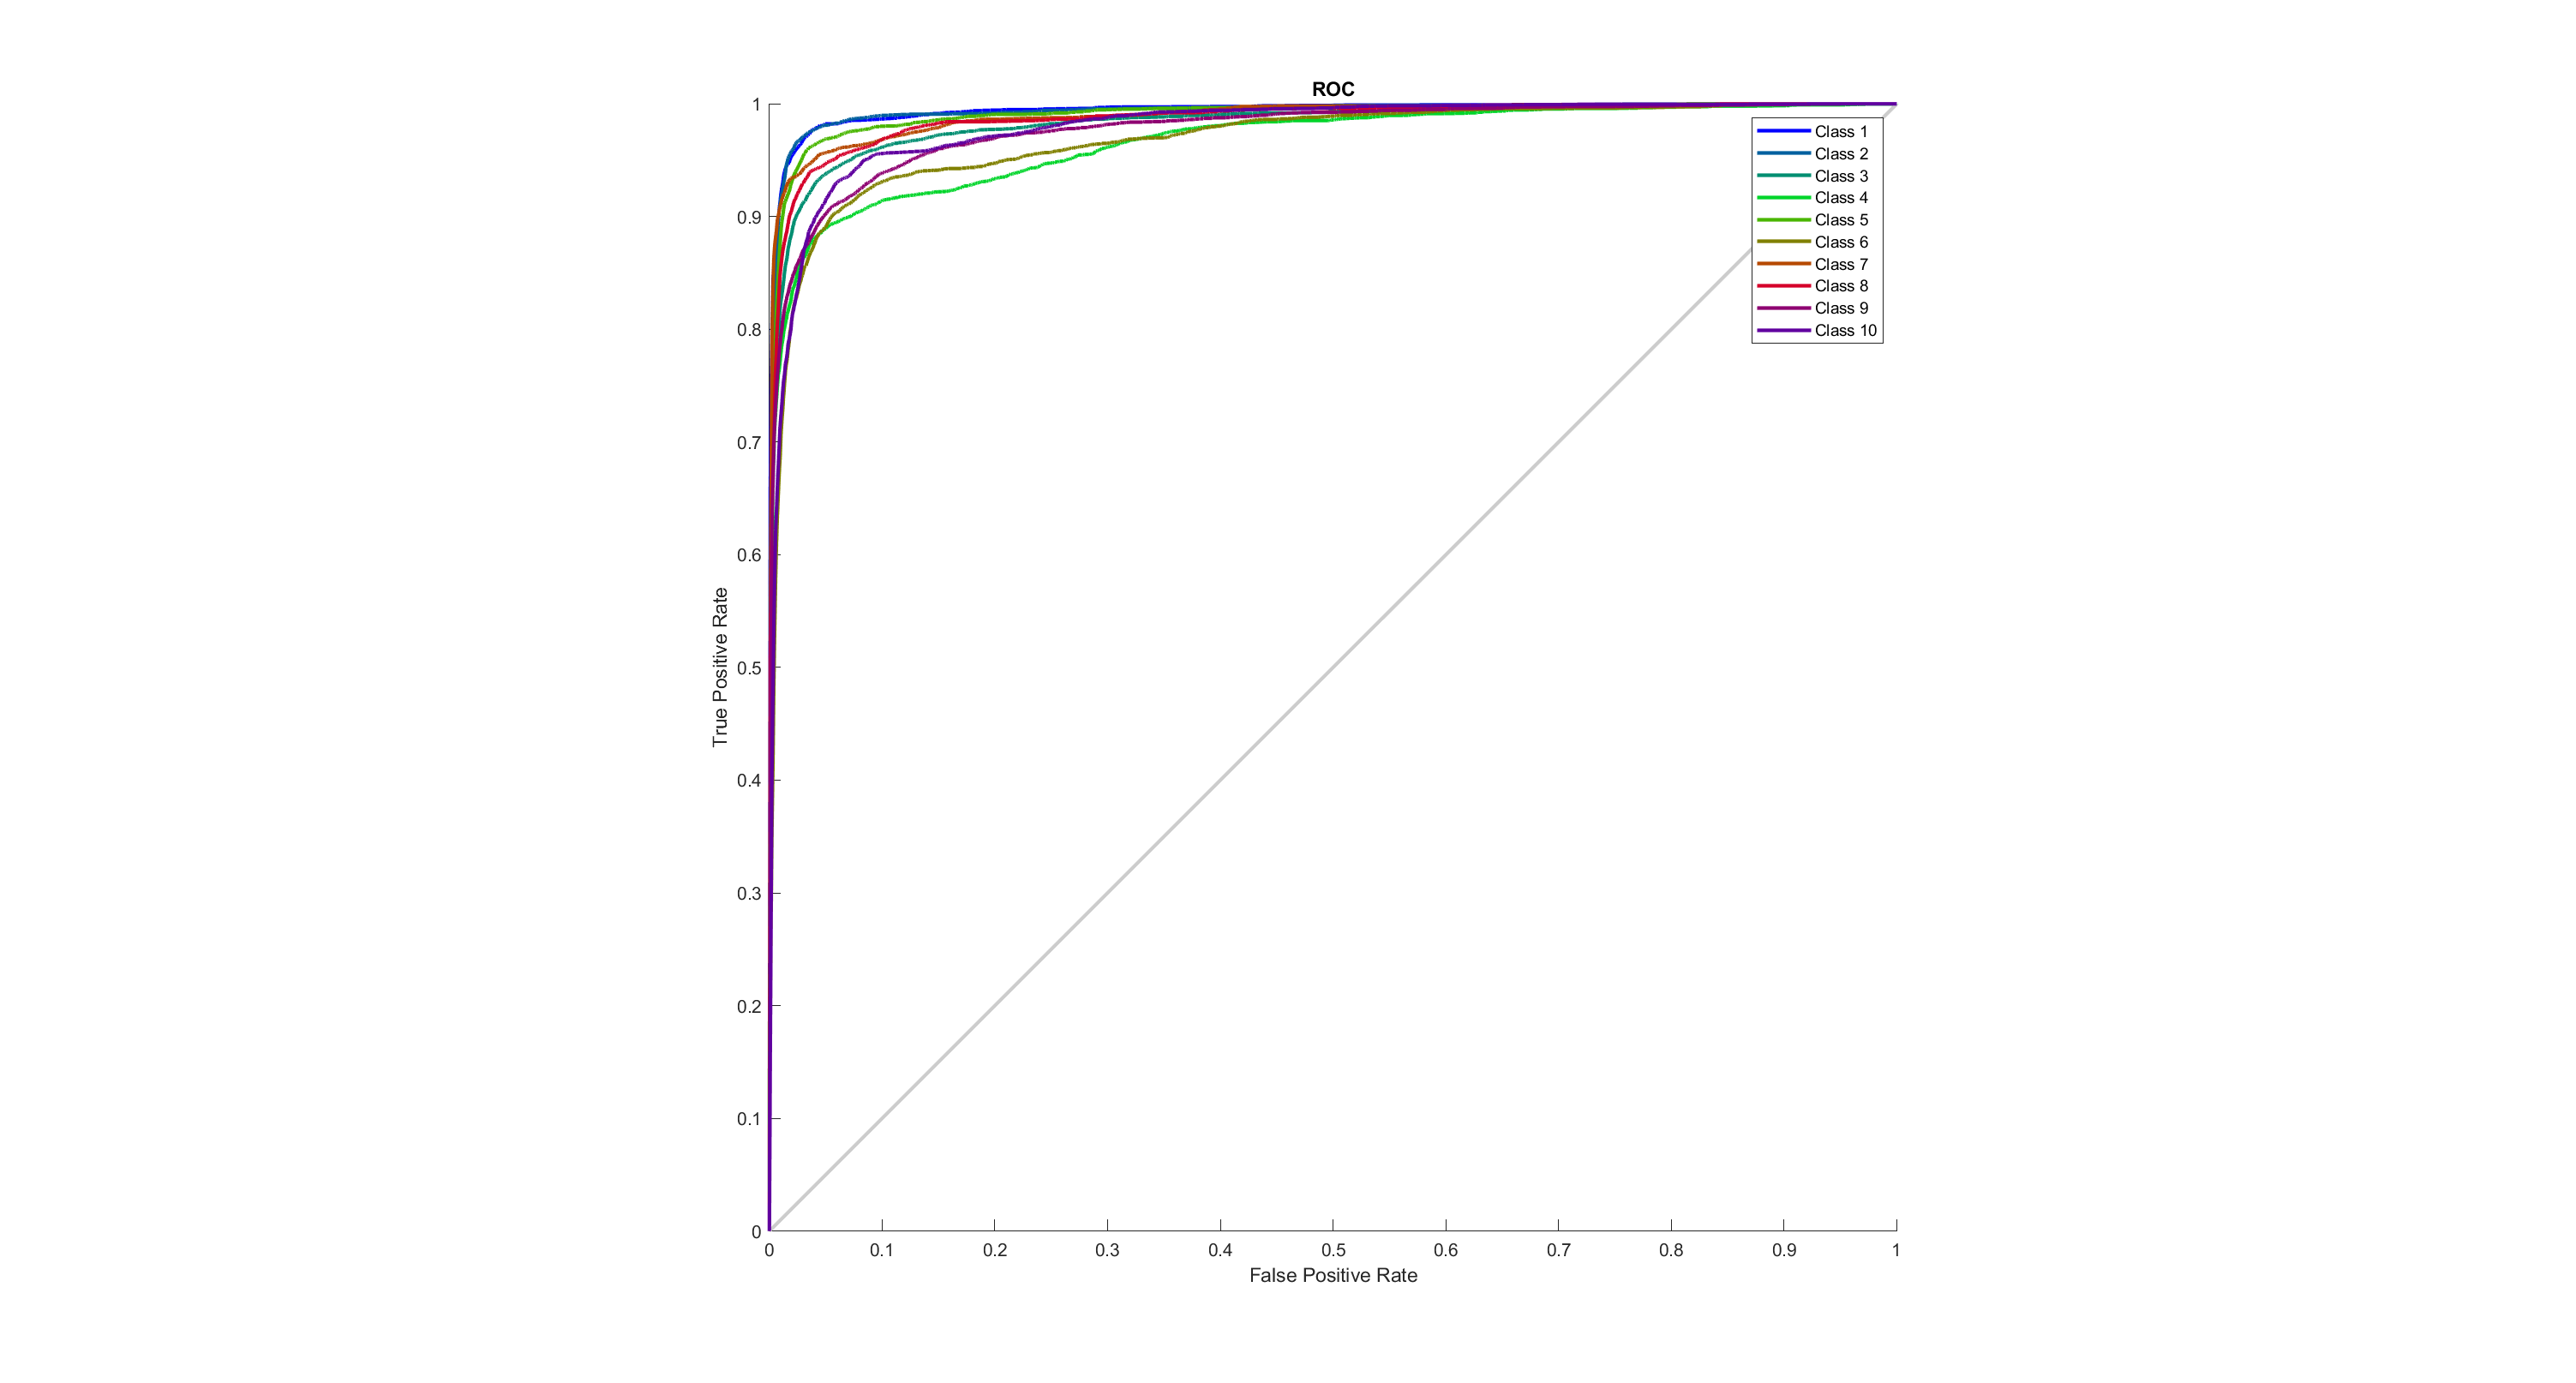
\includegraphics[width = 1.0\linewidth]{src1/ROC_5.png}
            \caption{ROC curve with 5 hidden nodes}
        \end{figure}
        \begin{figure}[H]
            \centering
            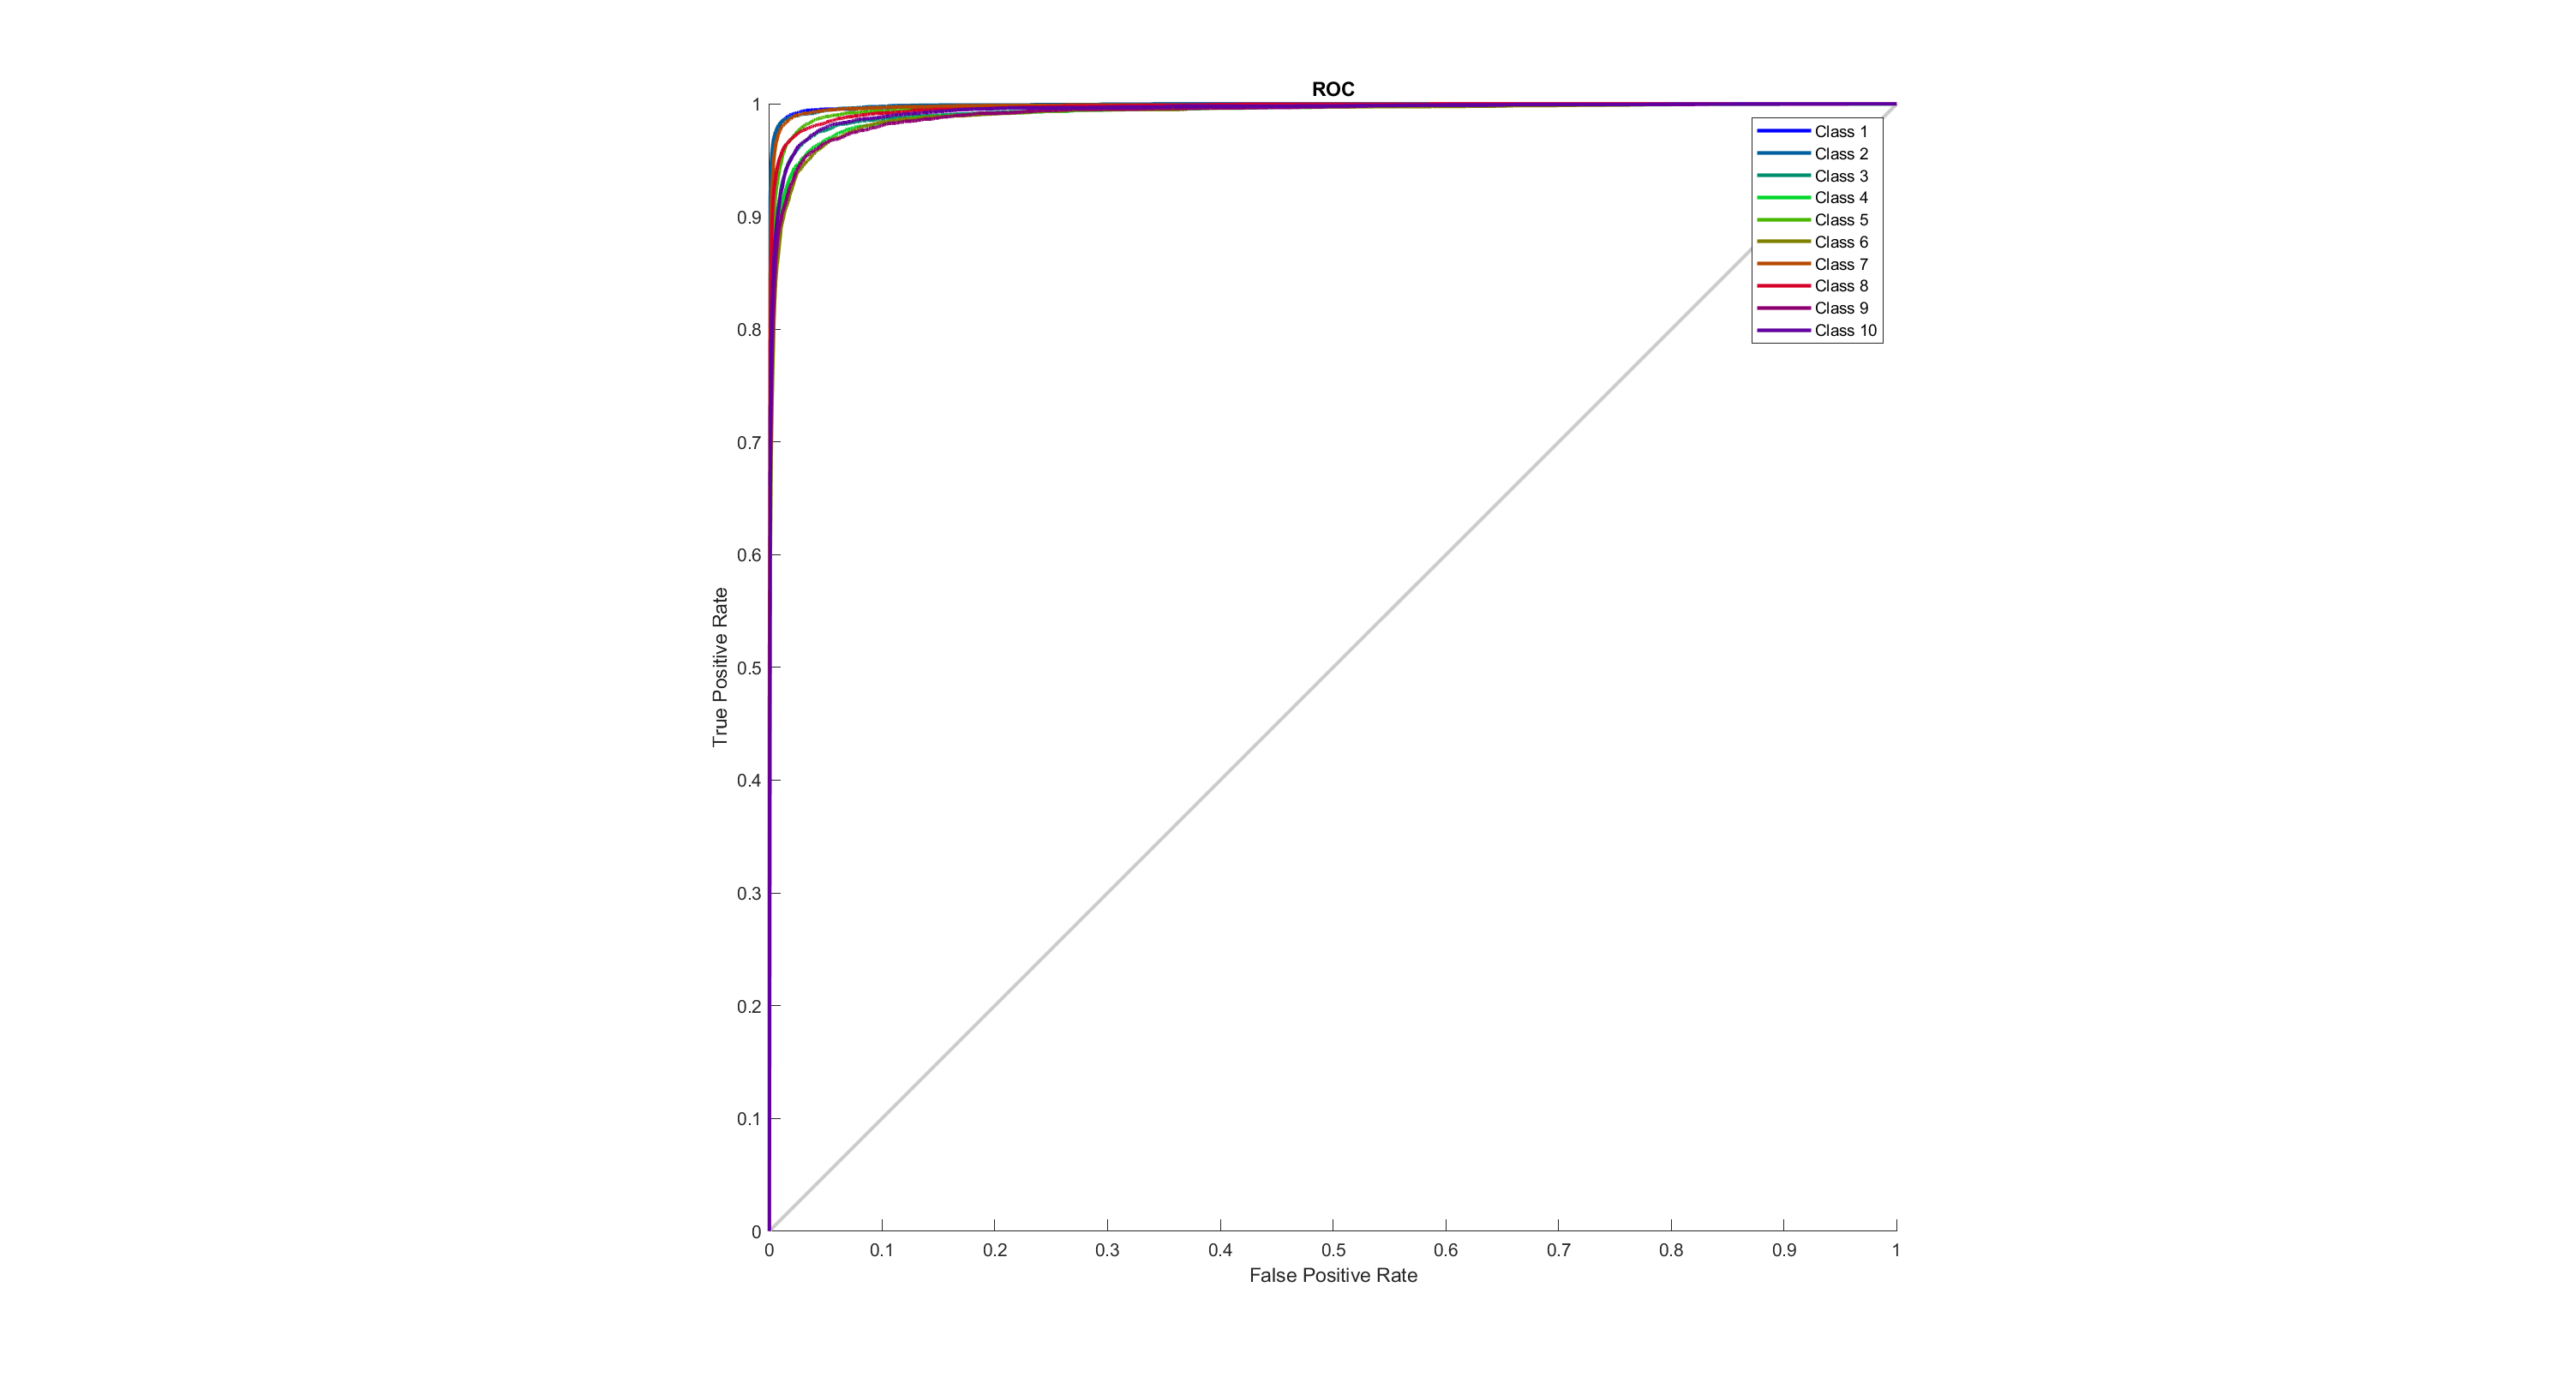
\includegraphics[width = 1.0\linewidth]{src1/ROC_10.png}
            \caption{ROC curve with 10 hidden nodes}
        \end{figure}
        \begin{figure}[H]
            \centering
            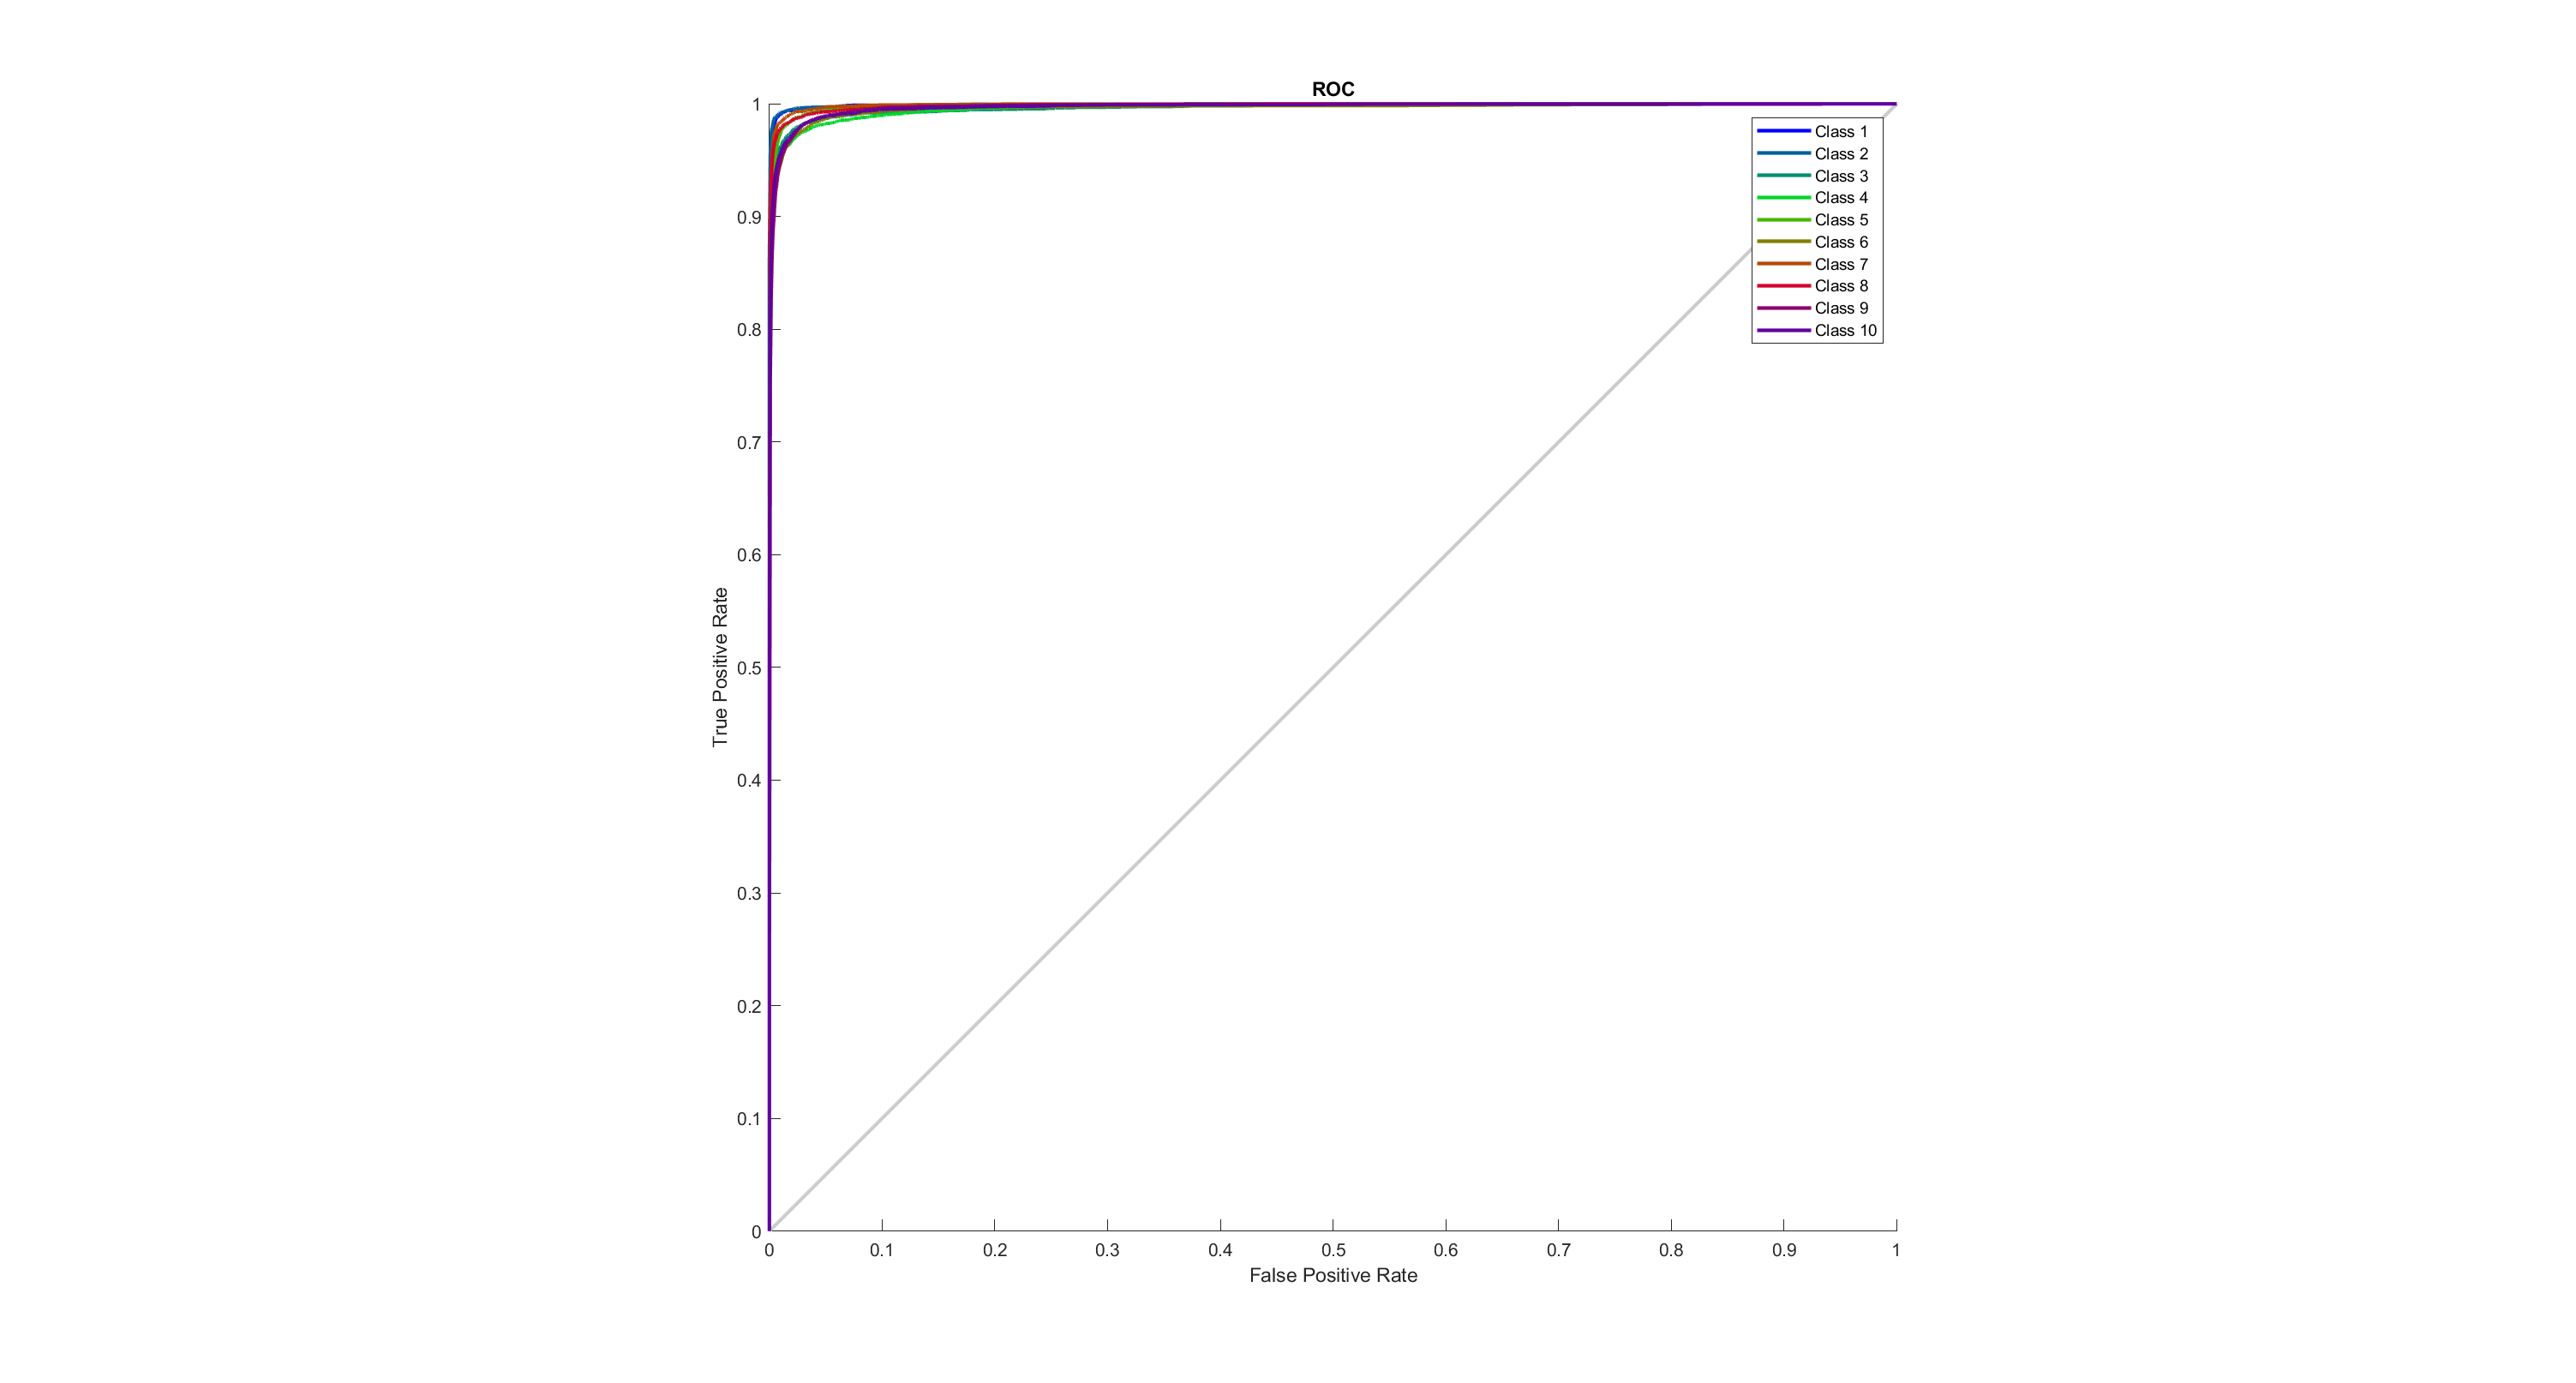
\includegraphics[width = 1.0\linewidth]{src1/ROC_20.png}
            \caption{ROC curve with 20 hidden nodes}
        \end{figure}
        \begin{figure}[H]
            \centering
            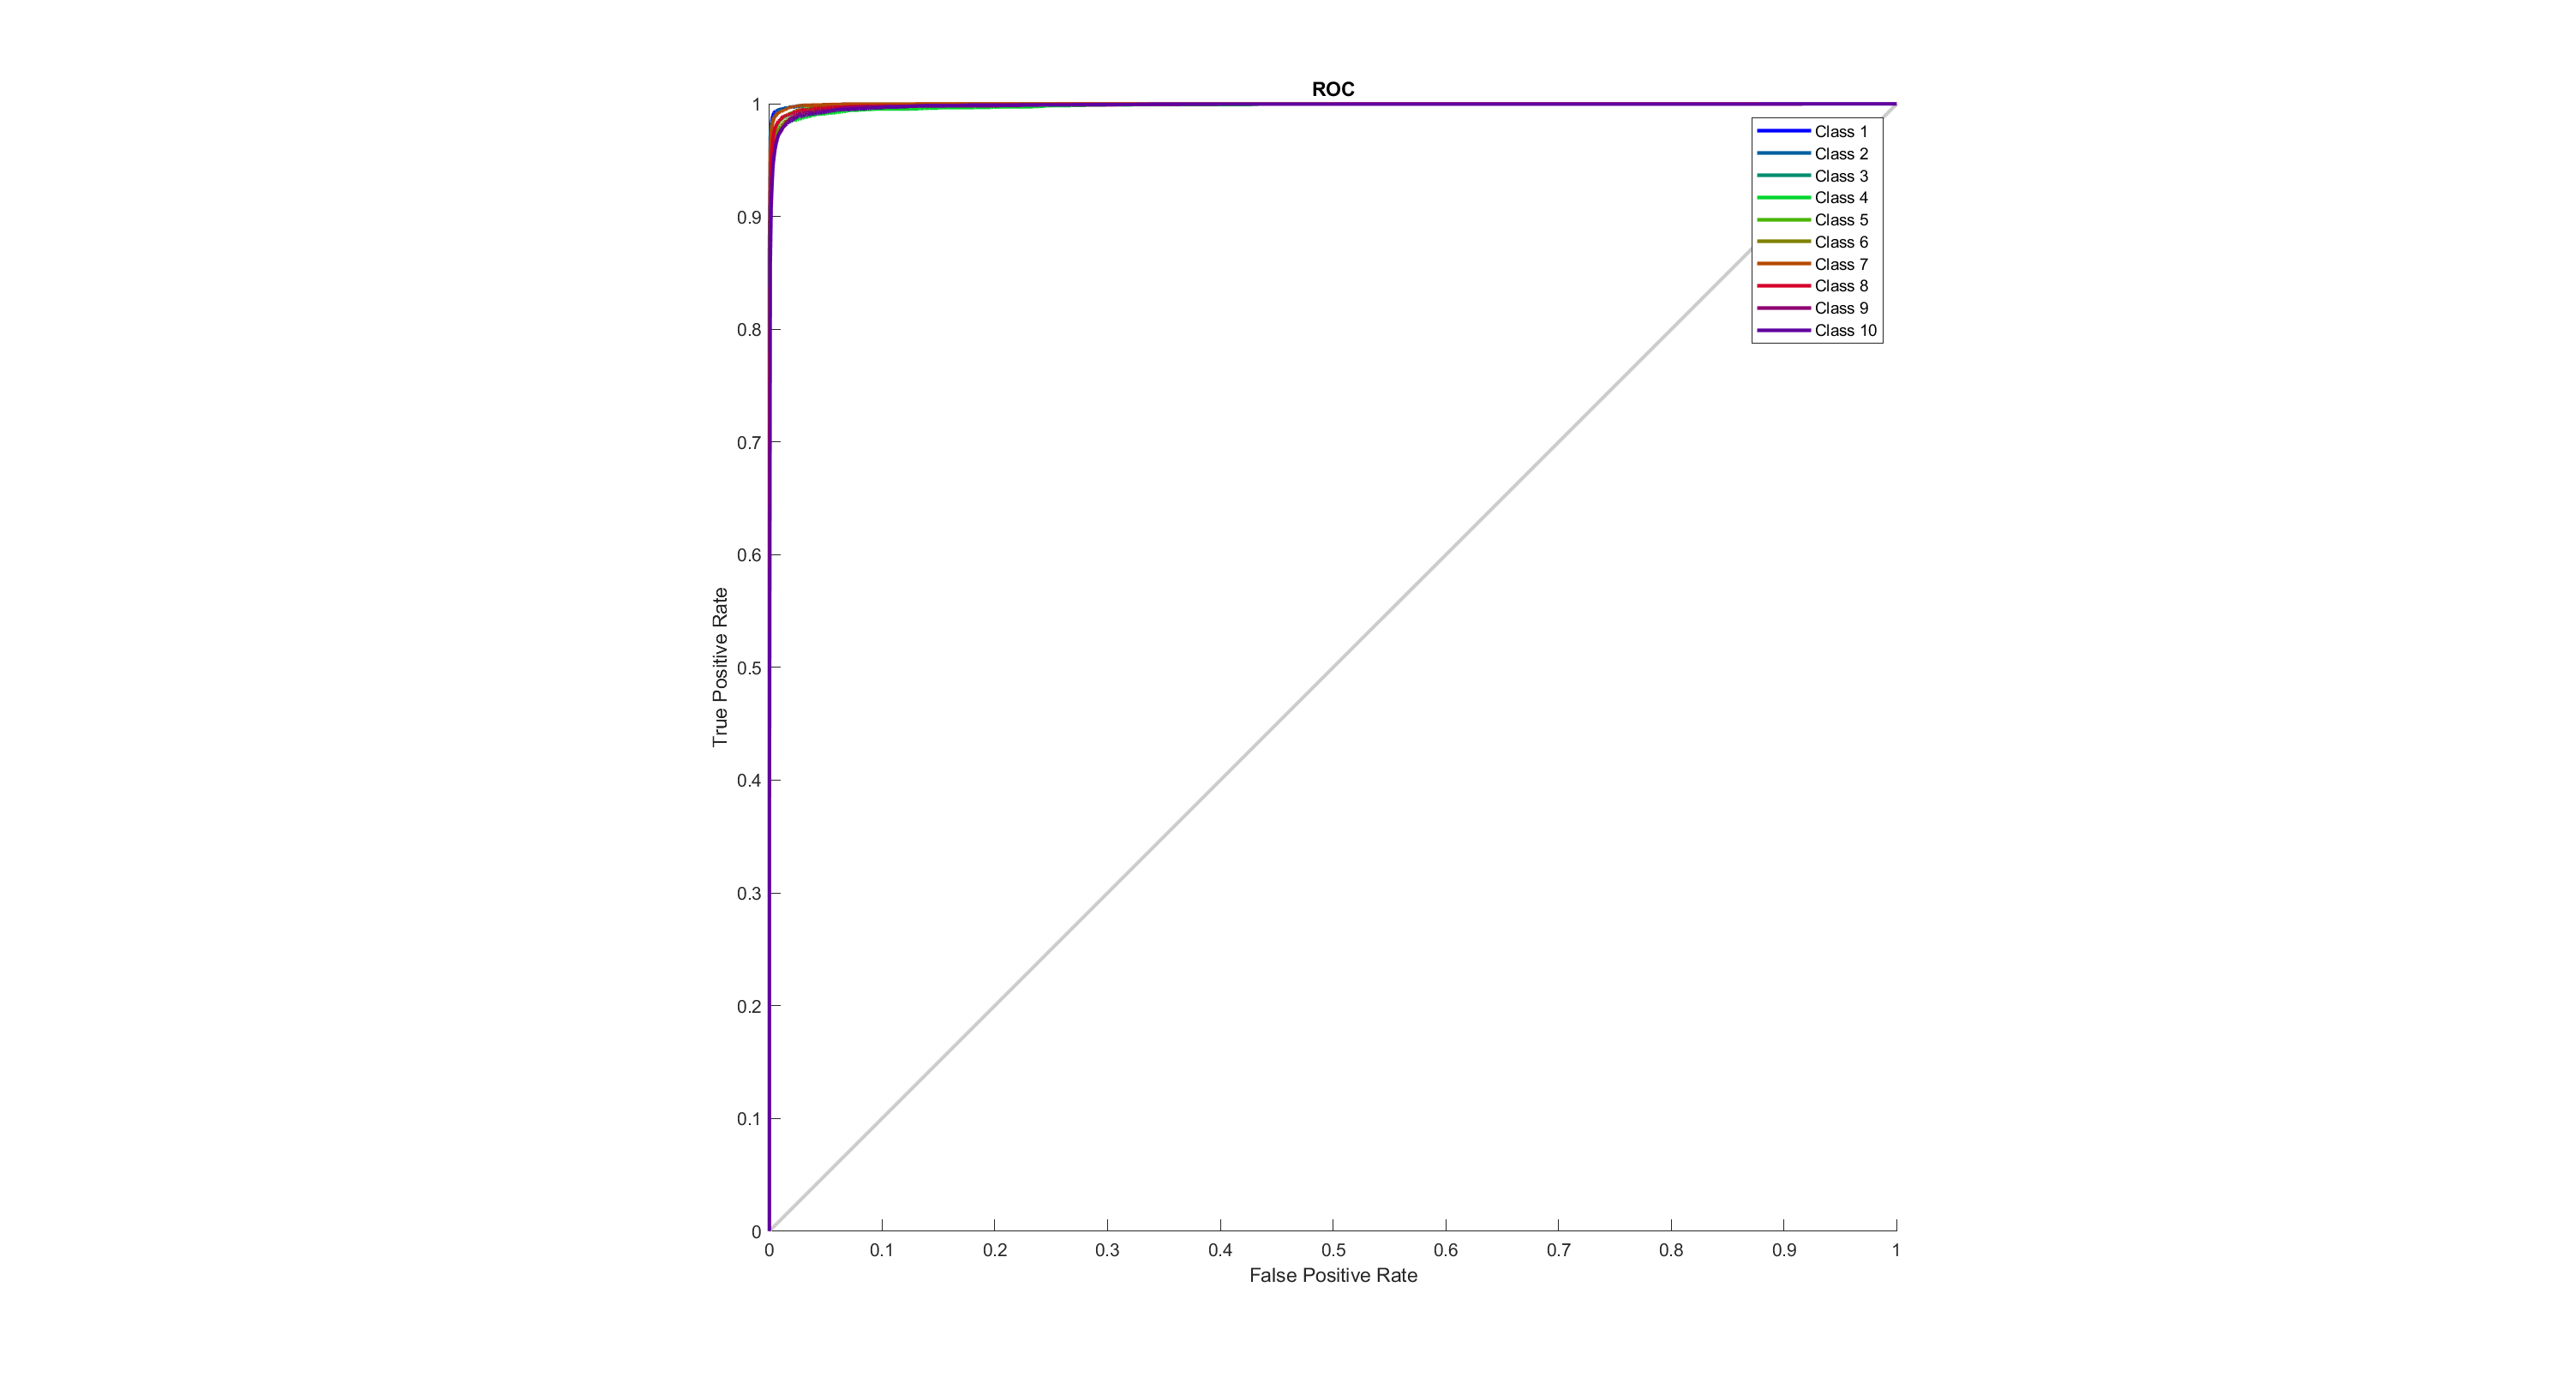
\includegraphics[width = 1.0\linewidth]{src1/ROC_40.png}
            \caption{ROC curve with 40 hidden nodes}
        \end{figure}
        \begin{figure}[H]
            \centering
            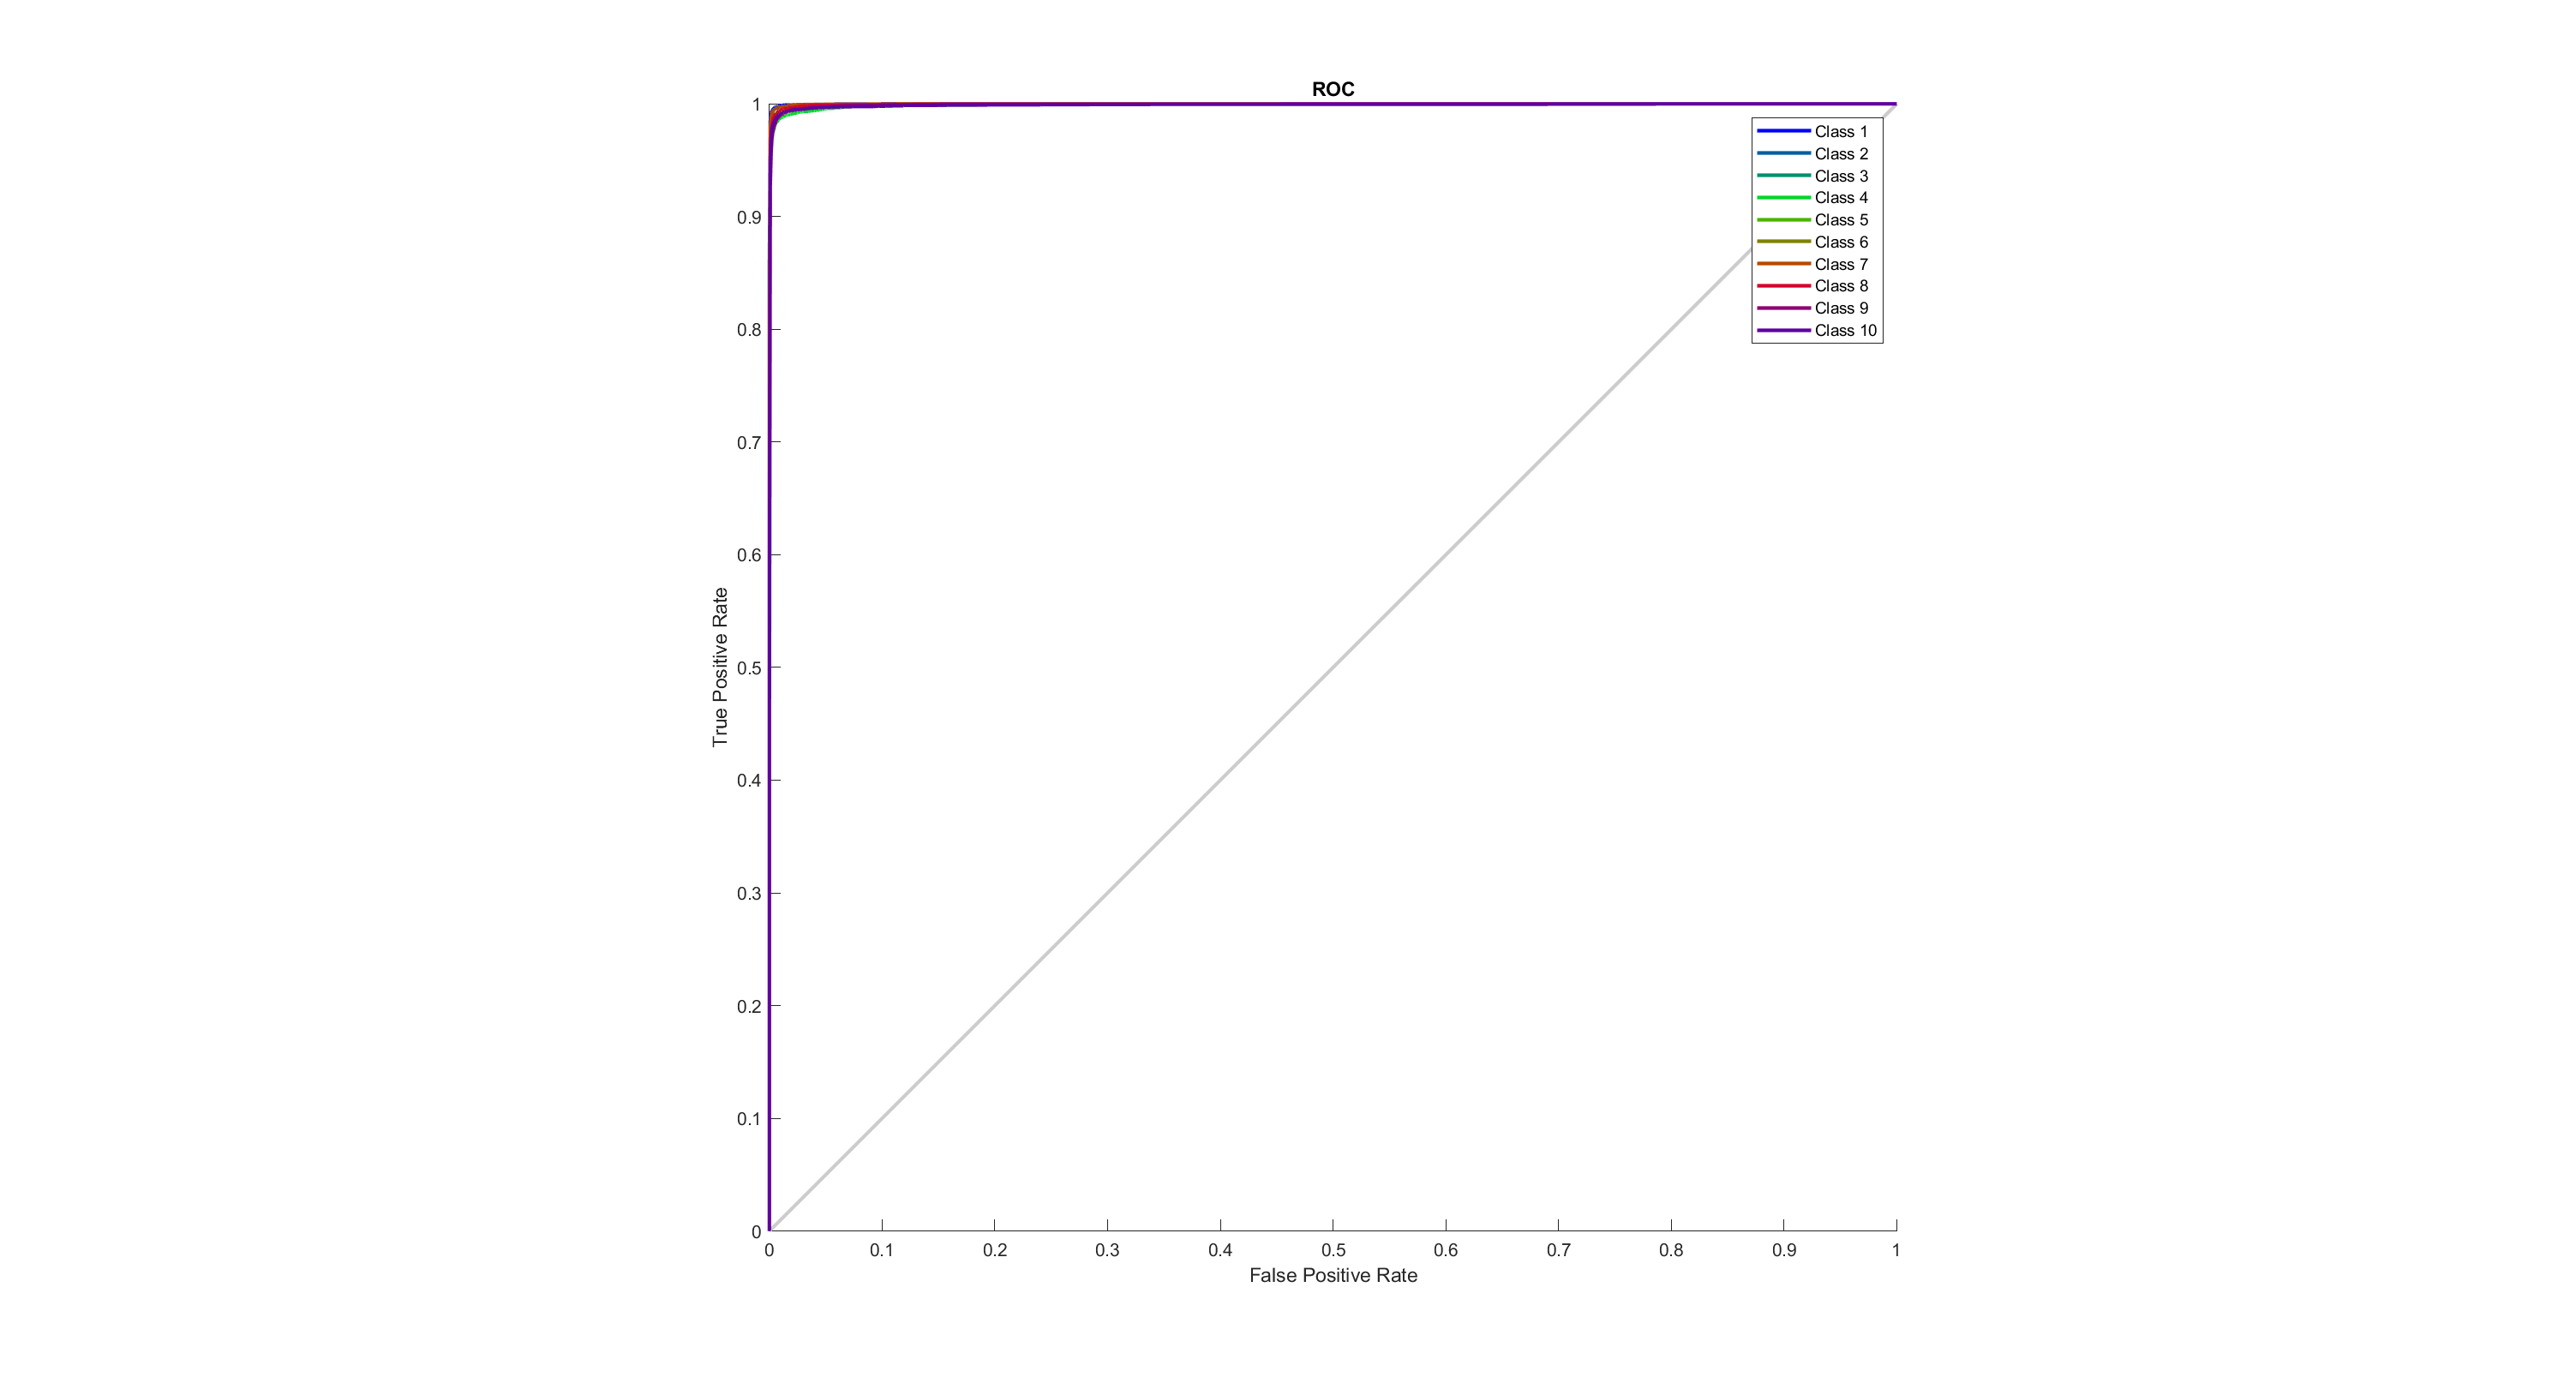
\includegraphics[width = 1.0\linewidth]{src1/ROC_100.png}
            \caption{ROC curve with 100 hidden nodes}
        \end{figure}
    }
    
    \subsection*{Conclusion}
    {
        \begin{itemize}
            \item \textbf{Confusion matrix:}\quad With more hidden nodes, the confusion rate drops accordingly. See the table below. 
            \begin{table}[htb!]
                \centering
                \begin{tabular}{|c|c|}
                \hline
                Hidden nodes & Total confusion rate \\
                \hline
                5 & 11.5\% \\
                \hline
                10 & 8.9\% \\
                \hline
                20 & 5.6\% \\
                \hline
                40 & 2.9\% \\
                \hline
                100 & 1.9\% \\
                \hline
                \end{tabular}
                \caption{Confusion rates}
            \end{table}

            \item \textbf{Performance:}\quad With more hidden nodes, the error rates drop at both validation set and testing set. Meanwhile, it takes a longer time before it stops and converges, in spite of fewer iterations. Another interpretation: The network has better capability of fitting the pattern with more hidden nodes, and therefore the training process is smoother and we need fewer iterations in training. But it takes more time since we have much more parameters to train, which leads to a longer time for each iteration step. 
            \begin{table}[htb!]
                \centering
                \begin{tabular}{|c|c|}
                \hline
                Hidden nodes & Total training epochs \\
                \hline
                5 & 500 \\
                \hline
                10 & 185 \\
                \hline
                20 & 125 \\
                \hline
                40 & 125 \\
                \hline
                100 & 110 \\
                \hline
                \end{tabular}
                \caption{Training iterations}
            \end{table}

            \item \textbf{ROC curve:}\quad With more hidden nodes, the ROC curve is closer to the left top corner, which indicates a better performance of classification. 

            
        \end{itemize}
    }

    \subsection*{Max Confusion}
    {
        \begin{figure}[H]
            \centering
            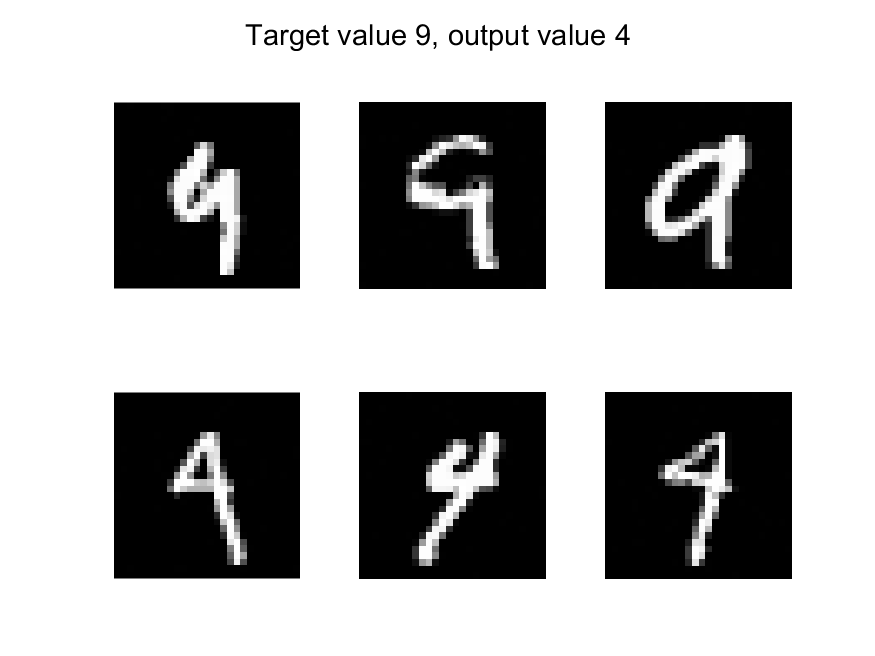
\includegraphics[width = 0.7\linewidth]{src1/max_confusion.png}
            \caption{Max confusion at target value ``4'', which is mistakenly output as ``9''}
        \end{figure}
    }
}

\section*{Question 2.1}
{
        \begin{lstlisting}[language=MATLAB]

    target_size = [patchsize, patchsize, 1];
    source_size = size(IMAGES);
    indices = [randi(source_size(1) - target_size(1) + 1, [1, numpatches]); ...
        randi(source_size(2) - target_size(2) + 1, [1, numpatches]); ...
        randi(source_size(3) - target_size(3) + 1, [1, numpatches])];
    for i = 1 : numpatches
        t = indices(:, i)';
        temp = IMAGES(t(1) : (t(1) + target_size(1) - 1), ...
            t(2) : (t(2) + target_size(2) - 1), ...
            t(3) : (t(3) + target_size(3) - 1));
        patches(:, i) = reshape(temp, [numel(temp), 1]);
    end

        \end{lstlisting}
}

\section*{Question 2.2}
{
    The sizes of $W_1$, $w_1$, $W_2$ and $w_2$ are, respectively, $25\times 64$, $25\times 1$, $64\times 25$ and $64\times 1$. Every line of code is vectorized.

    \begin{lstlisting}[language=MATLAB]

    N = size(data, 2);
    x_0 = data;                % 64-by-N
    
    z_1 = W1 * data + w1;      % 25-by-N
    x_1 = sigmoid(z_1);        % 25-by-N
    
    z_2 = W2 * x_1 + w2;       % 64-by-N
    x_2 = sigmoid(z_2);        % 64-by-N
    
    % Forward propagation
    
    J = 1/2 * sumsqr(x_2 - x_0) / N;
    R = lambda/2 * (sumsqr(W1) + sumsqr(W2));
    rho_hat = mean(x_1, 2);    % 25-by-1
    rho = sparsityParam;
    S = beta * sum( rho*log(rho./rho_hat) + (1-rho)*log((1-rho)./(1-rho_hat)) );
    
    cost = J + R + S;
    
    % Back propagation
    
    delta_2 = (x_2 - x_0) .* x_2 .* (1 - x_2);                    % 64-by-N
    
    W2grad = (delta_2 * x_1') / N + lambda * W2;                  % 64-by-25
    w2grad = mean(delta_2, 2);                                    % 64-by-1
    
    rhograd_2 = beta * ( - rho./rho_hat + (1-rho)./(1-rho_hat) );
    
    rhograd_1 = (x_1 .* (1 - x_1)) * x_0' / N;
    
    rhograd_0 = mean(x_1 .* (1 - x_1), 2);
    
    delta_1 = (W2' * delta_2) .* x_1 .* (1 - x_1);                % 25-by-N
    
    W1grad = (delta_1 * x_0') / N + lambda * W1 + rhograd_2 .* rhograd_1; % 25-by-64
    w1grad = mean(delta_1, 2) + rhograd_2 .* rhograd_0;           % 25-by-1

    \end{lstlisting}
}

\section*{Question 2.3}
{
    \subsection*{(1)}
    {
        Note that $S$ does not depend on $z_i^2$, we obtain
        $$\delta_i^2 = \frac{\partial}{\partial z_i^2} {\left[ \frac{1}{2} \sum_{j=1}^{n}{(f(z_j^2) - x_j)^2} + S \right]} $$
        $$= (f(z_i^2) - x_i) \frac{\partial}{\partial z_i^2} {f(z_i^2)} $$
        $$= (f(z_i^2) - x_i) \cdot f(z_i^2) (1 - f(z_i^2))$$
        $$= (\hat{x}_i - x_i) \cdot \hat{x}_i (1 - \hat{x}_i)$$ 
        where $$f(z_i^2) = x_i^2 = \hat{x}_i = \frac{1}{1 + \exp{(-z_i^2)}} = \left[ 1 + \exp{(- w_0^2 - \sum_{j=1}^{n_1}{W_{ji}^2 x_j^1})} \right]^{-1}.$$
    }

    \subsection*{(2)}
    {
        By definition, the simple gradient descent algorithm uses the iterations below:
        $$W_{ij}^1 \leftarrow W_{ij}^1 - \alpha \frac{\partial J}{\partial W_{ij}^1},$$
        $$w_0^2 \leftarrow w_0^2 - \alpha \frac{\partial J}{\partial w_0^2},$$
        where $\alpha$ is the learning rate with the gradients 
        $$\frac{\partial J}{\partial W_{ij}^1} = \frac{\partial J_s}{\partial z_j^1} \frac{\partial z_j^1}{\partial W_{ij}^1} + \frac{\partial R}{\partial W_{ij}^1} = d_j^1 x_i + \lambda W_{ij}^1,$$
        $$\frac{\partial J}{\partial w_0^2} = \frac{\partial J_s}{\partial z_j^2} \frac{\partial z_j^2}{\partial w_0^2} + \frac{\partial R}{\partial w_0^2} = d_j^2.$$
    }

    \subsection*{(3)}
    {
        By chain rule of multivariate derivatives, we obtain
        $$\delta_i^1 = \frac{\partial J}{\partial z_i^1} = \frac{\partial J}{\partial x_i^1} \frac{\partial x_i^1}{\partial z_i^1}$$
        $$= \frac{\partial J}{\partial x_i^1} \cdot x_i^1 (1 - x_i^1)$$
        $$= \left[ \frac{\partial J_s}{\partial x_i^1} + \frac{\partial S}{\partial x_i^1} \right] \cdot x_i^1 (1 - x_i^1)$$
        $$= \left[ \sum_{j=1}^{n_1}{\frac{\partial J_s}{\partial z_j^2} \frac{\partial z_j^2}{\partial x_i^1}} + \frac{\partial S}{\partial x_i^1} \right] \cdot x_i^1 (1 - x_i^1)$$
        $$= \left[ \sum_{j=1}^{n_1}{\delta_j^2 W_{ij}^2} + \frac{\partial S}{\partial x_i^1} \right] \cdot x_i^1 (1 - x_i^1),$$
        where $$\frac{\partial S}{\partial x_i^1} = \frac{\partial S}{\partial \hat{\rho}_i} = \beta \left( -\frac{\rho}{\hat{\rho}_i} + \frac{1 - \rho}{1 - \hat{\rho}_i} \right).$$
    }
}

\section*{Question 2.4}
{
    Given the hint, it is acceptable not to use vectorized manipulations here.

    \begin{lstlisting}[language=MATLAB]

    eps = 1e-6;
    for i = 1 : length(theta)
        dtheta = zeros(size(theta));
        dtheta(i) = eps;
        numgrad(i) = (J(theta + dtheta) - J(theta - dtheta)) / (2*eps);
    end

    \end{lstlisting}

    Run ``Step 3'' in ``train.m'', and the output indicates that the numerical and the analytical gradients correspond. The error is about $10^{-11}$.
    \begin{lstlisting}

    38.0000   38.0000
    12.0000   12.0000
    
    The above two columns you get should be very similar.
    (Left-Your Numerical Gradient, Right-Analytical Gradient)
    
    2.1452e-12
    
    Norm of the difference between numerical and analytical gradient (should be < 1e-9)

    8.2413e-11

    \end{lstlisting}

}

\section*{Question 2.5}
{
    Thanks to the vectorized expressions, the training process takes only 30 seconds before it stops at 400 iterations. The final cost is $0.4440$ with all paramters at default value.
}

\section*{Question 2.6}
{
    \begin{figure}[H]
        \centering
        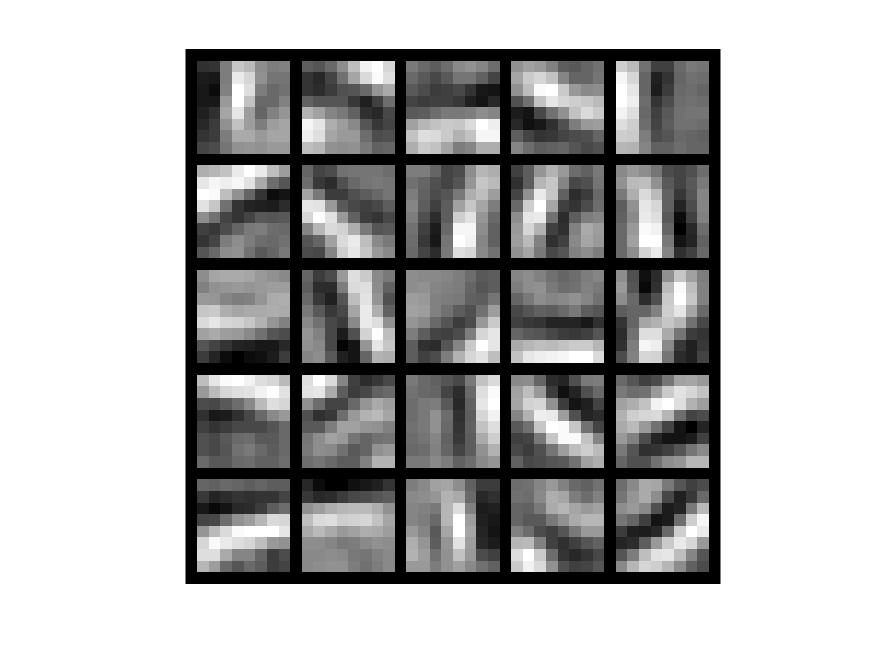
\includegraphics[width = 0.7\linewidth]{src2/weights.jpg}
        \caption{Visualization of the weights}
    \end{figure}
}

\section*{Source Code}
{
    Please download the souece code from http://39.106.23.58/files/PR4\_2015011506.7z

    For Question 1, please ``cd ./src1'' and run ``main.m''. It may take minutes to train the network, but the result is reproducible because of the random seed.

    For Question 2, please ``cd ./src2'' and run ``train.m'' by section.
}

\clearpage
\end{document}
    